\documentclass[a4paper,11pt]{article}
\usepackage{graphicx}
\usepackage{blindtext}
\usepackage[textwidth=17cm, top=1.5cm, bottom=1.5cm]{geometry}
\usepackage{array}
\usepackage[hidelinks]{hyperref}
\usepackage[nottoc,notlot,notlof,numbib]{tocbibind}
\usepackage{comment}
\usepackage{verbatim}
\usepackage{titlesec}
\usepackage{longtable}
\usepackage{float}
\usepackage[T1]{fontenc}
\usepackage[most]{tcolorbox}


\definecolor{warncolor}{rgb}{1, 0.95, 0.7}
\newtcolorbox{ibox}[1]{colback=warncolor,colframe=red!75!black,fonttitle=\bfseries,grow to right by=-10mm,grow to left by=-10mm, boxrule=2pt,boxsep=0pt,breakable}
\newcommand{\caution}[1]{\begin{ibox} \textbf{CAUTION:} \emph{#1} \end{ibox}}


\setlength{\parindent}{0pt}
\raggedright
\renewcommand*{\thesection}{\arabic{section}}
\titleformat{\paragraph}
{\normalfont\normalsize\bfseries}{\theparagraph}{1em}{}
\titlespacing*{\paragraph}
{0pt}{3.25ex plus 1ex minus .2ex}{1.5ex plus .2ex}

\setcounter{secnumdepth}{5}
\setcounter{tocdepth}{5}

\begin{document}

\title{DLT Viewer User Manual}
\author{Gernot Wirschal \textless Gernot.Wirschal@bmw.de \textgreater }


\maketitle

\begin{center}
( Alexander Wenzel, Simon Brandner, Lassi Marttala, Sven Hassler ) \linebreak
\end{center}

Changelog:\linebreak
v1.0.1, March 2020: add sort by timestamp and filetransfer autosave documentation\linebreak
v1.0.0, July 2019: adjust for 2.19.0 Release\linebreak
v0.0.7, February 2019: added UDP reception\linebreak
v0.0.6, Septemnber 2018: added logelevels, complete missing descriptions, bugfixing \linebreak
v0.0.5, June 2018: converted to \LaTeX, extended documentation, based on version 2.19.0 Release \linebreak
v0.0.4, February 2016: Updates and improvements for current DLT Viewer state \linebreak
v0.0.3, April 2013: Added Filetransfer command line description \linebreak
v0.0.2, December 2012: Converted to asciidoc \linebreak

\vspace{3cm}

\begin{figure}[h]
    \centering
    
\includegraphics[width=0.6\textwidth]{images/genivi_transparent.png}
\end{figure}

\pagebreak

\tableofcontents

\pagebreak


%##################################################################################################
%##################################################################################################
\section{Introduction}

\subsection{Purpose}


The DLT Viewer tool can decode, view and store DLT messages
generated by the DLT Daemon. The DLT Viewer tool enables the software developer and
the tester of the device to view and control the log and trace information. It is
not the goal of GENIVI to provide full functional analyzing tools for traces,
but to provide a basic set of utilities to visualize, control and test all features of the
DLT Daemon component in a simple way. The DLT Daemon component and the DLT Viewer
are based on the AUTOSAR 4.0 standard DLT.

We try to keep the GUI simple for an effective and efficient workflow, but also to
integrate as much functionality as needed.

%~~~~~~~~~~~~~~~~~~~~~~~~~~~~~~~~~~~~~~~~~~~~~~~~~~~~~~~~~~~~~~~~~~~~~~~~~~~~~~~~~~~~~~~~~~~~~~~~~~
\subsection{Restrictions and limitations}
The DLT Viewer once was created as an example application how to receive and display messages delivered by a DLT Daemon running on a
Linux DUT ( device under test ). Do not regard it as a perfect reference implementation.
The only existing requirement when starting the DLT Viewer development was "we need something like a DLT Viewer".
So depending on the used hardware ( RAM and hard disk size ), the amount of messages send by the daemon and the amount of connected
devices or the pure size of a logfile limits performance.


%~~~~~~~~~~~~~~~~~~~~~~~~~~~~~~~~~~~~~~~~~~~~~~~~~~~~~~~~~~~~~~~~~~~~~~~~~~~~~~~~~~~~~~~~~~~~~~~~~~
\subsection{Feature List}


\begin{itemize}
\item Graphical User Interface
  \begin{itemize}
    \item Menu and toolbar
    \item Project widget
    \item DLT Message Table
    \item Search results widget
    \item Status line with information about the current file etc.
  \end{itemize}
\item View DLT files
 \begin{itemize}
    \item Drag and Drop support
    \item Recent files selection
    \item Temporary files support
    \item Append files
    \item Index cache of already opened DLT files
    \item Default DLT file loading
    \item Open multiple files (v2.10.1)
 \end{itemize}
\item Retrieve DLT messages from targets and store them in DLT files
 \begin{itemize}
    \item Serial connections
    \item TCP/IP connections
    \item Multiple parallel connections
    \item Autoconnect to targets
    \item Configure log levels and trace status
    \item Store configuration in target
    \item Reset the target's configuration
    \item Organise connections in projects
 \end{itemize}
\item Filter DLT messsages for analysing
 \begin{itemize}
    \item Support to show only a defined subset of the messages
    \item Complex filter configurations
    \item Save and restore filter configurations
    \item Multiple default filter configurations
    \item Markers to highlight specific messages
    \item Filter index cache of already filtered DLT files
    \item Regular expressions
    \item Sorting by receive time (starting with v2.10.1)
 \end{itemize}
\item Clipboard support
 \begin{itemize}
    \item Copy selected DLT messages to clipboard
 \end{itemize}
\item Export of DLT files in multiple formats
 \begin{itemize}
    \item Supported formats:
     \begin{itemize}
       \item DLT format with selection
       \item ASCII format
       \item CSV format
     \end{itemize}
 \end{itemize}
\begin{itemize}
    \item Select the messages to be exported
       \begin{itemize}
       \item All messages
       \item Filtered messages
       \item Marked messages
     \end{itemize}
 \end{itemize}
\item Search DLT messages
   \begin{itemize}
    \item Step by step search
    \item Search export view
    \item Search by regular expressions
   \end{itemize}
\item Project configurations
   \begin{itemize}
    \item Control log levels
    \item Organise configurations in projects
    \item Save and restore projects
    \item Recent projects selection
    \item Select displayed columns
    \item Default project loading
    \item Automatic timezone synchronisation (v2.10.1)
   \end{itemize}
\item Plugin configurations
   \begin{itemize}
    \item Decoder plugins to decode messages
    \item Viewer plugins to show more detailed information and analyse logs. Viewer plugins provide extra widgets to visualize data
    \item Control plugins to control applications on the target
    \item Available plugins
     \begin{itemize}
        \item DLT Viewer Plugin
        \item Non Verbose Mode Plugin
        \item Filetransfer Plugin
        \item DLT Logstorage Config Creator Plugin ( outdated )
        \item DLT System Viewer Plugin ( outdated )
        \item DLT DBus plugin
     \end{itemize}
   \end{itemize}
\item Command line support
 \begin{itemize}
    \item Silent mode
    \item Loading project
    \item Loading DLT file
    \item Using filter configuration
    \item Export DLT files to ASCII
    \item Execute commands in plugins
 \end{itemize}
\item Plugins programming guide
\end{itemize}

\pagebreak

%##################################################################################################
\section{DLT Viewer GUI}

\subsection{Layout}

\begin{comment}
\begin{figure}[h]
 \centering
  \includegraphics[width=0.9\textwidth]{images/main_window_plain.png}\linebreak\linebreak
 \caption{Main DLT Window}
 \label{fig:maindltwindow}
\end{figure}
\end{comment}


The screenshot in \autoref{fig:mainwindowsections} will give you a quick impression about how the Viewer
could look. The Viewer is based on Qt, so there are widgets you can move
around and resize as you like. Your settings of position and size of the
widgets are stored when you close the Viewer so that you have exactly the
same window when you launch the Viewer the next time.
To get a better understanding about the DLT Viewer parts the screenshot
below marks the relevant areas followed by a description.

\nopagebreak
\begin{figure}[h]
 \centering
  %\includegraphics[width=1.1\textwidth]{images/main_window_annotated.png}
  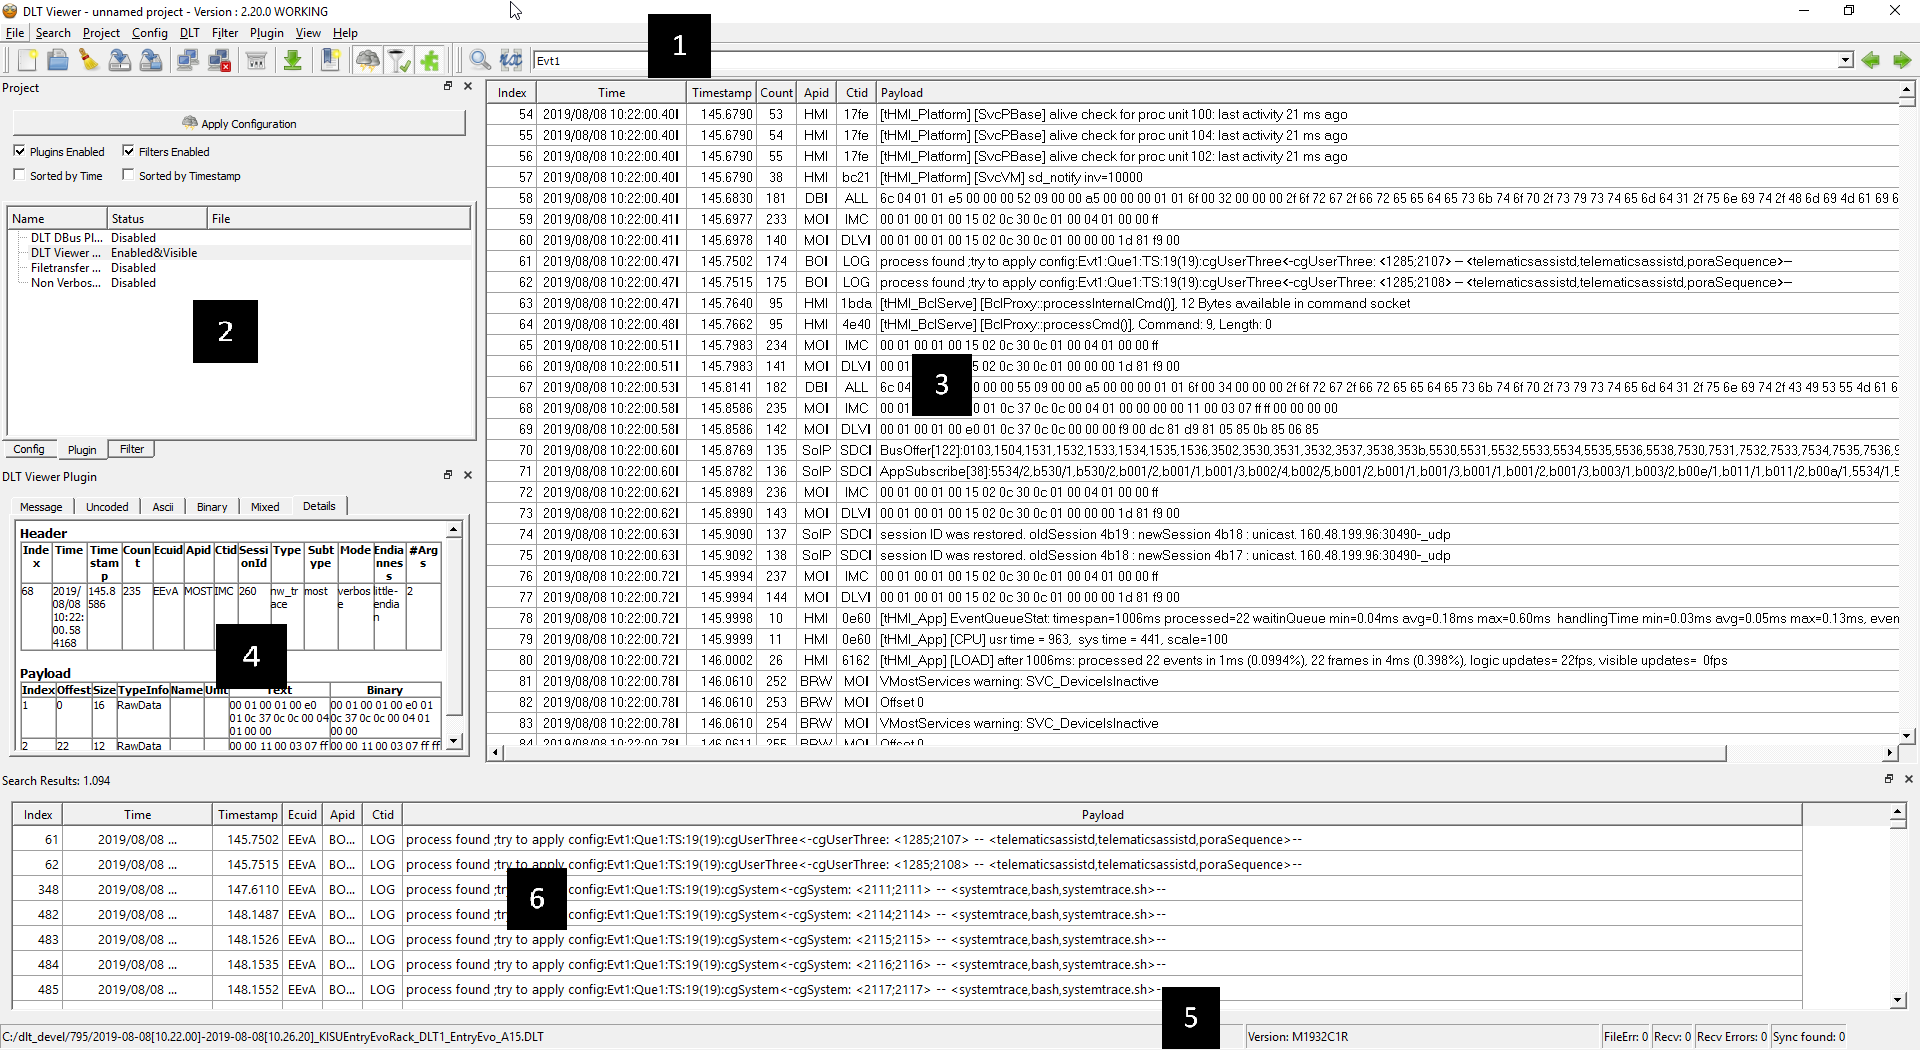
\includegraphics[width=1.1\textwidth]{images/dltviewermain_sections_annotated.png}
  \caption{Main DLT Window sections}
 \label{fig:mainwindowsections}
\end{figure}


%\begin{figure}[h]
% \centering
%  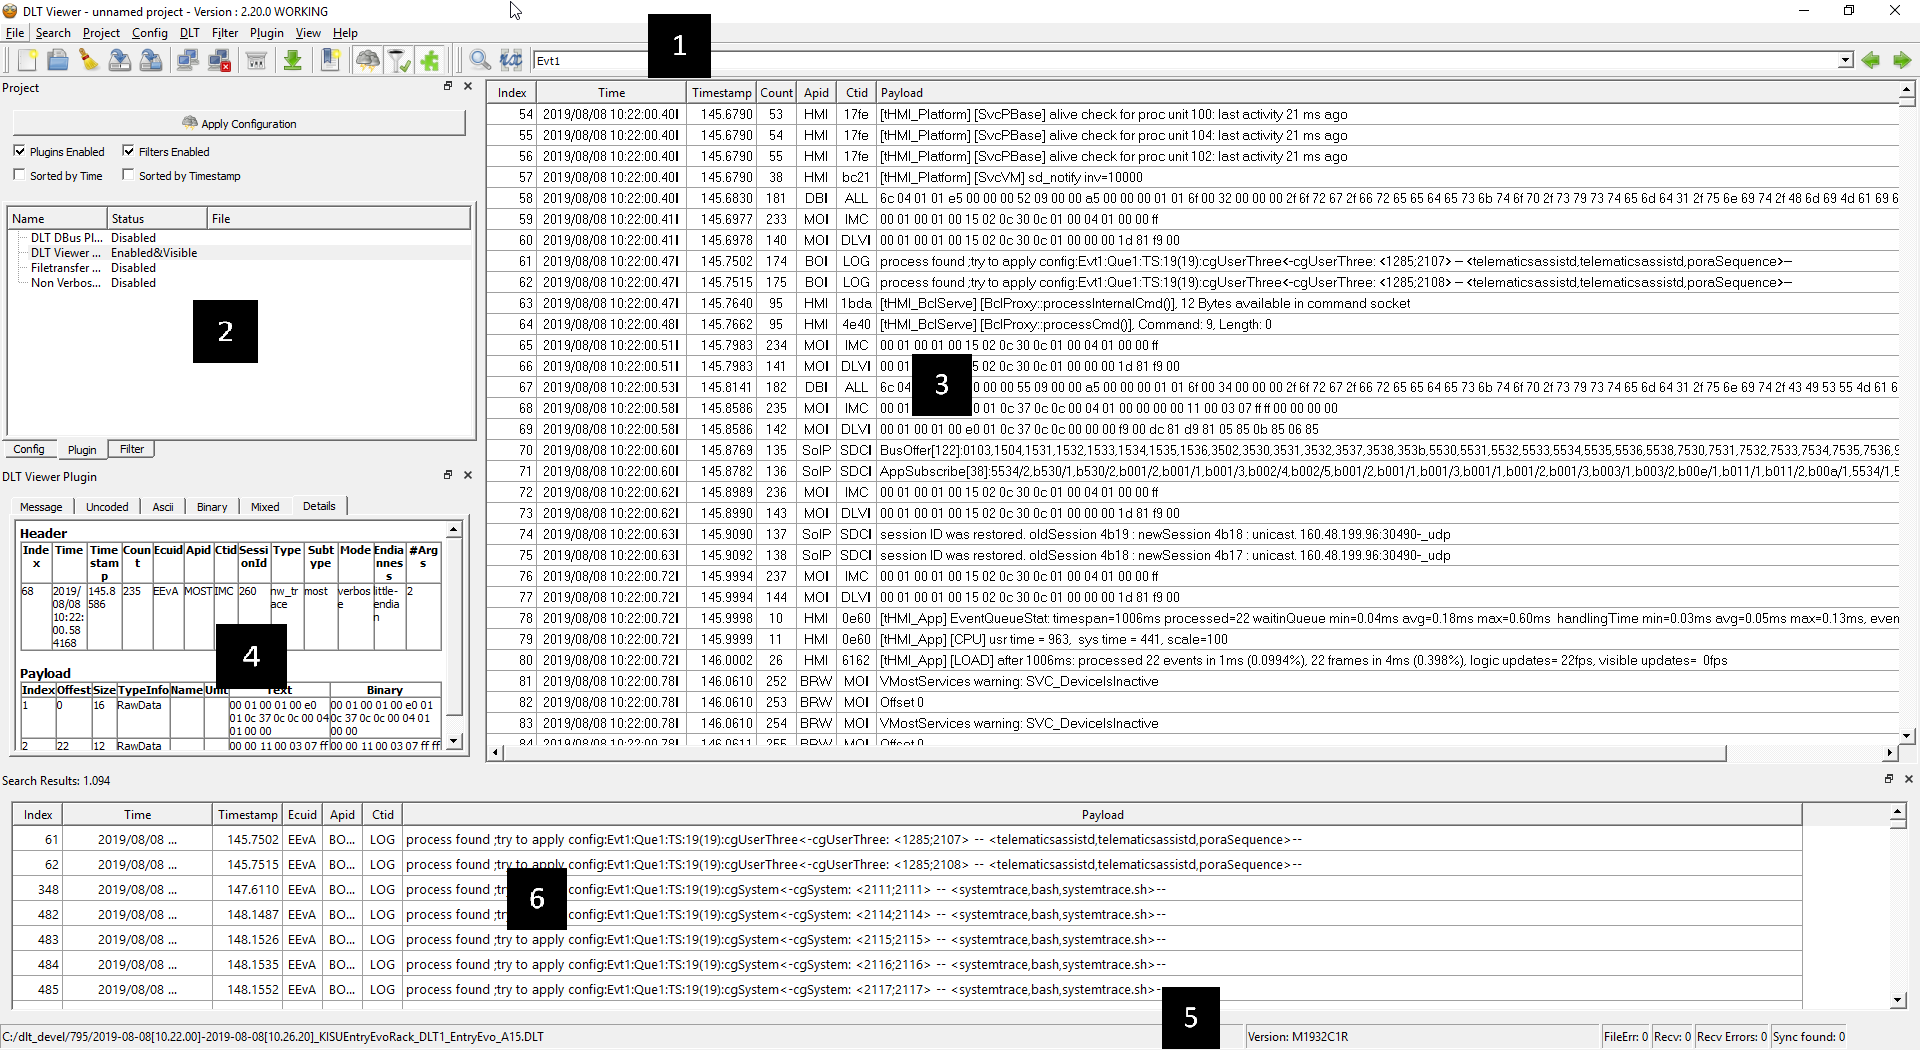
\includegraphics[width=1.1\textwidth]{images/dltviewermain_sections_annotated.png}
% \caption{Main DLT Window sections}
%\end{figure}


\pagebreak

\begin{longtable}{| l | m{3cm}  | m{11cm} |}
\caption[GUI section description]{GUI section description} \label{guisectiondescription} \\
 \hline
   \textbf{Nr} & \textbf{Title} & \textbf{Description} \\
\hline
%1 Zeile
   \includegraphics[width=0.05\textwidth]{images/Mark1.png}
   &
    Menu and Toolbar
   &
   In the window title you can find the absolute path of your project file 
   and the project name. If you start the DLT Viewer
   with no default project file it will
   create an unnamed project.

   The menu consists of:

\begin{itemize}
    \item \begin{bf}File\end{bf}
     Open and save files, access DLT Viewer settings etc.
    \item \begin{bf}Search\end{bf}
     Search for specific messages in the current log.
    \item \begin{bf}Project\end{bf}
      Create, open and save DLT Viewer projects.
    \item \begin{bf}Config\end{bf}
     Add, edit and remove ECUs, applications and contexts.
    \item \begin{bf}DLT\end{bf}
      Additional functions concerning the DLT daemon and the current configuration.
    \item \begin{bf}Filter\end{bf}
       Create, open and save filters for the message log.
    \item \begin{bf}Plugin\end{bf}
     Enable, show and edit plugins.
    \item \begin{bf}View\end{bf}
     Select the visible components of the DLT Viewer.
    \item \begin{bf}Help\end{bf}
    Get information and help for the DLT Viewer. Find here detailed version information, the support email address as well as
    an overview of the comandline options.
 \end{itemize}

The menu provides main functions to the user. Many menu functions are also easily accessible through the toolbar.
Hover the cursor over toolbar buttons to see their functions. \\
   \hline

%2 Zeile
   \includegraphics[width=0.05\textwidth]{images/Mark2.png}
   &
    Project Panel
   &
   The project widget allows you to configure and control the project,
   load an existing project, save a changed configuration to the DLT Daemon and
   more. The project panel is split into three tabs:
   \begin{itemize}
    \item The "Config" tab, which contains all connected ECUs/Devices.
     Each Device contains its connected applications.
     Each application contains its used contexts.
    \item The "Filter" tab lets you configure filters and markers,
    which are used to show or
    mark only a defined subset of DLT messages in the message table.
    \item The "Plugin" tab shows the available DLT Viewer plugins. The development team provides a
    plugin SDK to you. You are able to write your own DLT Viewer plugins to decode
    messages, display an extra GUI panel or control the Viewer and target applications.
   \end{itemize}

   In the settings you can e.g. select a default project, which is loaded during start-up.  \\
   \hline
   \includegraphics[width=0.05\textwidth]{images/Mark3.png}
   &
    DLT Message Table
   &
   In the DLT Message Table you see all DLT messages in the current DLT log file.
   Newly received DLT messages are written to the end of the log file.
   If the AutoScroll option is enabled in the settings, the table will scroll along with new DLT messages while they are received.
   The columns in the message table are:\label{messagetablecolumns}
  \begin{itemize}
   \item \begin{bf}Index\end{bf}
    Index of the DLT message in the DLT log file.
   \item \begin{bf}Time\end{bf}
    Time when the message was received.
   \item \begin{bf}Timestamp\end{bf}
     Time when the message was sent, measured since the startup of the target.
   \item \begin{bf}Count\end{bf}
    Cyclical counter, one per context. Can be used to detect lost messages.
   \item \begin{bf}Ecuid\end{bf}
    Name of the sending ECU. Defined in the "Projects" tab.
   \item \begin{bf}Apid\end{bf}
    Indetifier of the message sender application. Defined by the sending application.
   \item \begin{bf}Ctid\end{bf}
    Context indentifier of the message sender. Defined by the sending application.
   \item \begin{bf}Sessionid\end{bf}
    Process ID of the target process / application submitting the message.
   \item \begin{bf}Type\end{bf}
    Type of the message (Log / Trace).
   \item \begin{bf}Subtype\end{bf}
    Log level or trace type.
   \item \begin{bf}Mode\end{bf}
    Verbose or Non-Verbose.
   \item \begin{bf}Args\end{bf}
    The number of arguments in the payload of the message.
   \item \begin{bf}Payload\end{bf}
    The payload shows all parameters of the log message as text.
  \end{itemize}
If a filter is configured, you will see only DLT messages which match
this filter. Remove or disable all filters if you want to see all messages.
If there are decoder plugins and a DLT message matches one of these plugins, the decoded
payload is displayed instead of the raw payload.
DLT log files can be loaded and saved in the file menu.
 \\
   \hline
   \includegraphics[width=0.05\textwidth]{images/Mark4.png}
   & Plugin Widget
   & Provides one or more widgets to display additional data. You can choose which plugins are to be shown in the "Plugin" tab.
   See section \autoref{plugintab} and chapter \autoref{plugins} for more information.   \\
   \hline
   \includegraphics[width=0.05\textwidth]{images/Mark5.png}
   & Status line
   & \label{footer}The status line shows information about the current log file,
     the version string ( see \autoref{versionstring} ) and other options of the DLT Viewer. \\
   \hline
   \includegraphics[width=0.05\textwidth]{images/Mark6.png}
    & Search table
    & \label{searchtable}The search table shows all resulting lines of a search pattern as well as the amount of search hits \\
   \hline

\end{longtable}


\pagebreak

%~~~~~~~~~~~~~~~~~~~~~~~~~~~~~~~~~~~~~~~~~~~~~~~~~~~~~~~~~~~~~~~~~~~~~~~~~~~~~~~~~~~~~~~~~~~~~~~~~~
\subsection{Project Panel}

\subsubsection{Config Tab}


\begin{figure}[H]
 \centering
 \includegraphics[width=0.6\textwidth]{images/project_widget.png}
 \caption{Config Tab}
 \label{fig:configtab}
\end{figure}


In the config tab you can see a hierarchical list of all configured devices, applications and contexts.
\begin{comment}
\begin{itemize}
 \item The ECU item lists the ID of the ECU, its status (red = offline, yellow = connecting,green = online), a description of the ECU including the connection interface, the defaultlog level and the default trace status.
 \item The application item lists the ID and the description of the application.
 \item The context item lists the ID, the description, the log level and the trace status of the context.
 \item Double clicking an item lets you configure it. Right clicking an item gets you a context menu, depending on the type of the item:
\end{itemize}
\end{comment}

The ECU item lists the ID of the ECU, its status (red = offline, yellow = connecting,green = online), a description of the ECU including the connection interface, the defaultlog level and the default trace status.\linebreak
The application item lists the ID and the description of the application.\linebreak
The context item lists the ID, the description, the log level and the trace status of the context.
Double clicking an item lets you configure it. Right clicking an item gets you a context menu, depending on the type of the item:\linebreak

\vspace{0.3cm}

Right click on empty space to add a new ECU connection\linebreak

\vspace{0.1cm}

\includegraphics[width=0.2\textwidth]{images/ecu_add.png}\linebreak

\vspace{0.1cm} See \autoref{connecttoecu} on how to connect to an ECU.\linebreak

\vspace{0.3cm}

Right click on an ECU ( ECU Edit ) to change or configure ECU settings\linebreak

\vspace{0.1cm}

\includegraphics[width=0.2\textwidth]{images/ecu_context_menu.png}

\vspace{0.1cm}

Right click on an application to configure an application

\vspace{0.1cm}

\includegraphics[width=0.2\textwidth]{images/app_context_menu.png}

\vspace{0.1cm}

Right click on a context to configure a context\linebreak

\vspace{0.1cm}

\includegraphics[width=0.2\textwidth]{images/ctx_context_menu.png}

\vspace{0.1cm}


\subsubsection{Filter Tab}
The filter list gives you an overview of all configured filters. Only DLT messages which match the enabled filters are displayed in the message table view.
Double clicking a filter item lets you change the filter. Each filter can be customized to include or exclude messages, to check for
specific ECUs, applications or contexts, for header and payload content and more. It is also possible to create marker filters, which don't
include or exclude any messages but highlight them in a selected color.


\begin{figure}[H]
 \centering
 \includegraphics[width=0.6\textwidth]{images/filter_widget.png}
 \caption{Filter Tab}
 \label{fig:filtertab}
\end{figure}


By right clicking ( or select Menu bar \ensuremath{\rightarrow} Filter ) you get the following menu to add or change a filter:

\vspace{0.1cm}
\includegraphics[width=0.2\textwidth]{images/filter_context_menu.png}
\linebreak

"Save Filter" lets you store your filter configuration to a file with extension *.dlf.
Both the "Load Filter" and the "Append Filter" option will load a saved filter file, but "Load Filter" will reset your current filter list while appending keeps it.

The filters you set will apply to all incoming or loaded DLT messages. If you also want to apply the filters to previously logged messages, hit the
"Apply Configuration" button on the top of the "Filter" tab.

Seel also \autoref{workingwithfilters} for more information on how working with filters.

\paragraph{Filter Quickselect}
\label{filterquickselect}
%You can use the quick select bar to choose and enable your favourite filters placed in the default filter path ( see in Section "\ref{defaultfilterpath} Viewer Configuration Settings" ).
You can use the quick select bar to choose and enable your favourite filters placed in the default filter path.
The filters can be selected from the drop down list. If you place a new filter there, it will be recognized at start up or after pressing "Refresh".
To set the default filter path see also \autoref{defaultfilterpath}{ Viewer Configuration Settings }.

\begin{figure}[H]
 \centering
 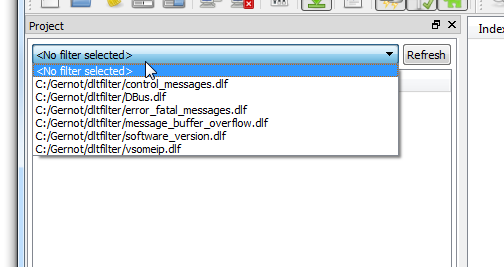
\includegraphics[width=0.6\textwidth]{images/selectfilter.png}
 \caption{Filter quickselect}
 \label{fig:filterquickselect}
\end{figure}


\subsubsection{Plugin Tab}
\label{plugintab}
The plugin list shows all loaded plugins.
Plugins e.g. can be used to:
\begin{itemize}
 \item decode DLT messages
 \item provide additional graphical widgets
 \item control the viewer
 \item send injection messages to target applications
 \item control any attached measurement equipement like USB or IEC devices
\end{itemize}

Double clicking on a plugin item creates a popup window which lets you enable/disable the plugin and select a configuration file for it. On more informnation for the plugins see chapter \autoref{plugins}.

\begin{figure}[H]
 \centering
 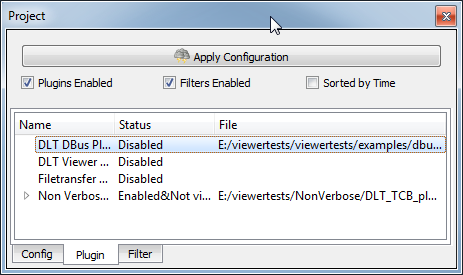
\includegraphics[width=0.6\textwidth]{images/plugin_tab.png}
 \caption{Plugin Tab}
 \label{fig:plugintab}
\end{figure}



\begin{itemize}
 \item The "Name" column shows the name of each plugin. This name is provided by the plugin itself.
 %\item The "Interface" column tells you the type of the plugin (or more precisely: what interfaces it implements). For each plugin this column shows a combination of "View", "Decode", "Ctrl" and "Command".
 \item The "Status" column shows which plugins are enabled and visible. Only plugins that implement the "View" interface can have the status "Visible".
 %\item The "Info" column lists the number of description items for each plugin. The description items can be seen by expanding plugin items that have an arrow next to them.
 \item The "File" column tells you the path of the configuration file or files for plugins that have such a file or files selected. Double click on plugin items to choose configuration files for them.
\end{itemize}

%~~~~~~~~~~~~~~~~~~~~~~~~~~~~~~~~~~~~~~~~~~~~~~~~~~~~~~~~~~~~~~~~~~~~~~~~~~~~~~~~~~~~~~~~~~~~~~~~~~~~~~

\pagebreak
\subsection{Viewer Configuration Settings}
Access via "File \ensuremath{\rightarrow} Settings Menu".
\linebreak
Set general behaviour of the viewer like temp file locations.

\nopagebreak


\subsubsection{Global Settings}
\label{globalsettings}
Here the "file behaviour" like e.g. locations and usage of log files or index files can be configured.

\begin{figure}[H]
 \centering
 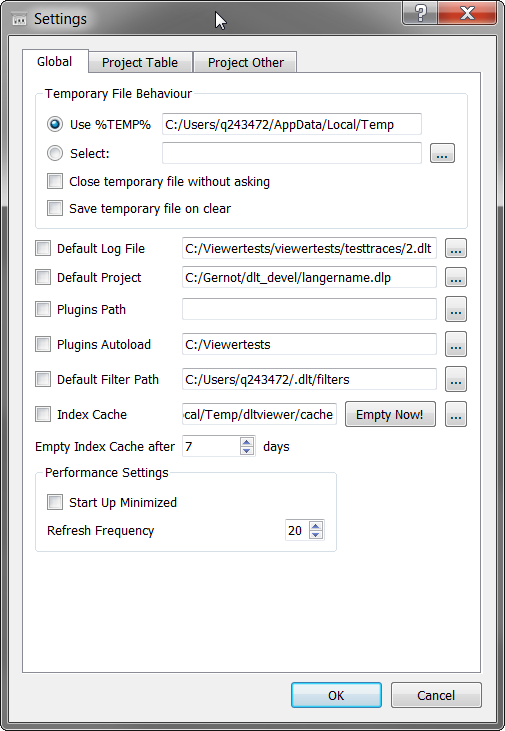
\includegraphics[width=0.6\textwidth]{images/settings_global.png}
 \caption{Global Settings Tab}
 \label{fig:globalsettingstab}
\end{figure}


Here find some selected descriptions:

\begin{enumerate}
\item{Temporary File Behaviour}

\label{temporaryfile}
In "Temporary File Behaviour" you can set some parameters concerning the temporary file
which is always created during live tracing.
You can just use the system default location or define a custom folder of your choice.

\caution{Keep in mind that in case "Save temporary file on clear" is selected the amount of files in your tmp path increases
and your hard disk will easily run out of space. So take care about this temp path !}

\item{Default log File}

If enabled, the given log file will always be opened instead of creating a new tmp file at Viewer startup.
Live tracing messages are appended to this file.
The changes to this setting take place the next time the viewer is started. In case the file does not exist it is created.

\caution{In case you do not remove/change the logfile e.g. in an automated setup, it may easily increase and cause the viewer to take a long time loading the file
at next start !}

\item{Default Project}

\label{defaultproject}
If enabled, the given project file will always be opened at viewer startup. The settings in the project file rules
the default viewer configuration settings.
The changes to this setting take place the next time the viewer is started.
On project files see \autoref{projectfiles}.


\item{Plugins Path}

\label{pluginspath}
If enabled the viewer will look for plugins in this location additionaly to the default locations.
See also \autoref{installremoveplugins}.

\item{Plugins Autoload}

\label{enableautoload}
If the plugins autoload path is enabled and set accordingly you can make use of the plugin autoload feature.
\linebreak
On details how to use plugins autoload see \autoref{usingautoload}

\item{Default Filter Path}

\label{defaultfilterpath}
If the default filter path is enabled and set accordingly you can use the "Filter quick select bar" in the Filter Tab.
Also see \autoref{filterquickselect}{ Filter Quickselect }.
\nopagebreak

\item{Index Cache}

When the index cache is enabled, reloading of previous loaded files is much faster because the index is cached in additional files.
To reduce disk space consumption these files can be automatically deleted after the specified amount of days of last access.
The deleting takes place the next time the viewer is started. The index files have the extension "*.dix" and are located in the specified folder.
\caution{If this option is enabled, additional disk space is used. Take care to observe the size of the index file directory, especially in case you perform 
         frequent comandline conversions e.g. in an automated setup. So it is recommended to disable index caching for commandline usage. }

\item{Performance Settings}

When "Start up Minimized" is enabled the viewer window is not shown diretly. Most propably makes sense when using logging only mode.

The Refresh Frequency specifies the amount of viewer GUI refreshes per second.
\end{enumerate}


%-------------------------------------------------------------------------------
\subsubsection{Project Table Settings}

\begin{figure}[H]
 \centering
 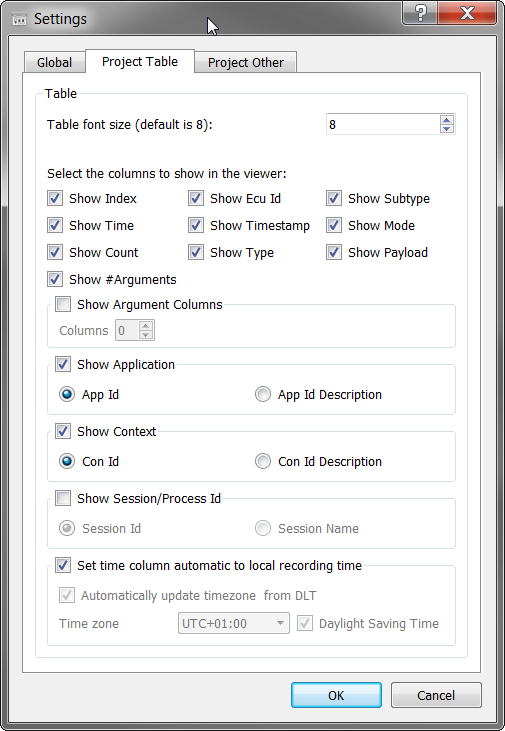
\includegraphics[width=0.6\textwidth]{images/settings_projecttable.png}
 \caption{Project Table Tab}
 \label{fig:projecttabletab}
\end{figure}

\nopagebreak

\begin{enumerate}
\item{Table font size}

Here you can set the desired font size to be used in the message table view, the default font size is 8.

\item{Select columns to show in the viewer}

In the this settings tab you mainly can select which columns you want to have displayed in the table view.
See also \autoref{messagetablecolumns} on information about the columns.

\item{Show Arguments}

This setting may be only interesting for dlt application developers. The column "Args" shows the number of payload arguments contained in the DLT message.

The check box "Show Argument Columns" is not functional.

\item{Show Application}

Select if the Apid shall be shown, if so you can choose the Apid itself or the description string which comes with the application registration message.

\item{Show Context}

Select if the Ctid shall be shown, if so you can choose the Ctid itself or the description string which comes with the context registration message.

\item{Show Session/Process Id}

Process ID of the target process submitting the message. "Session Name" only is available if transmited by the daemon.

\item{Set time column automatic to local recording time}

Here you can choose which time for the receive time column should be used. You can just take local time of the system
or use the DLT time settings by choosing the time zone and the mode of daylight saving time.
\end{enumerate}


\subsubsection{Project Other Settings}

General logging behaviour configurations

\begin{figure}[H]
 \centering
 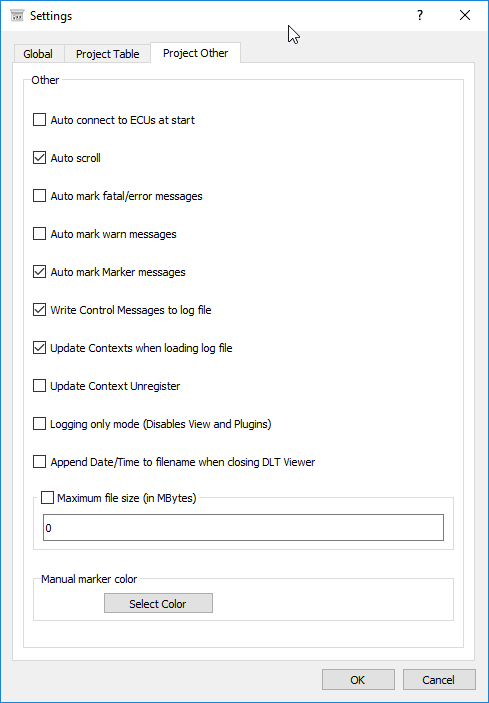
\includegraphics[width=0.6\textwidth]{images/settings_other.png}
 \caption{Project Other tab}
 \label{fig:projectotherab}
\end{figure}

Some choosen settings:


\begin{enumerate}

\item{Auto connect to ECUs at start}

If this chechbox is enabled the last ECU connected is tried to be connected automatically.
In case you are using a project file this setting may be overruled !

\item{Auto scroll}

\item{Auto mark fatal/error messages}

Automatically mark all messages of subtype ( loglevel ) "fatal" and "error" with red color.

Note: in case you use a filter using a marker the filter overcolor rules this setting.

\item{Auto mark warn messages}
Automatically mark all messages of subtype ( loglevel ) "warn" with yellow color.

Note: in case you use a filter using a marker, the filter color overrules this setting.


\item{Auto mark marker messages}

\label{automarkmarker}
Automatically mark all marker messages with green color.

Note: in case you use a filter using a marker, the filter color overrules this setting.

Example:

\includegraphics[width=0.8\textwidth]{images/markermessage.png}

\item{Write Control Messages to Log File}
\label{controlmessagestolog}
When this checkbox is enabled, control messages like register or unregister of applications or contexts, SW version and get\_log\_info from the daemon are displayed
in the message table and stored in the logfile.

\item{Update Contexts when loading Log file }

The list of contexts is updated automatically when a log file is loaded.


\item{Update Contexts Unregister}

The list of contexts is updated automatically when a context is deleted.


\item{Logging only mode}
\label{enableloggingonlymode}
When enabling this check box you activate the "logging only" mode, see \autoref{Loggingonlymode}:

\item{Append Date/Time to filename when closing DLT Viewer}

The time when the DLT Viewer is closed is appended to the current logfile name.
Of course this implies that you did save the temprorary log file to a custom file before as the tmp file
usually is not saved ...
Here also the log file files gets a name appendix of type \begin{verbatim} __YYYYMMDD_hhmmss____YYYYMMDD_hhmmss \end{verbatim} specifying the start receive time stamp and the end receive time stamp of the log.


\item{Maximum File Size}

The logfile is split up in several files of given maximum size in [MB].
The files get a name appendix of type \begin{verbatim} __YYYYMMDD_hhmmss____YYYYMMDD_hhmmss \end{verbatim} specifying the start receive time stamp
and the end receive time stamp of the log.
So later you can also concatenate the files to a single one in the right order.

E.g.:
\begin{verbatim}
cat *.dlt >> combine.dlt
\end{verbatim}

\caution{Depending on the message traffic and the choosen split file size there may occur a message loss in case the split file size is to small ( < 10 kb )}

\item{Manual marker color}

Select your favourite color for marking selected lines in the table view.
Right mouse click on the table view to highlight the selected lines. Marking only has a visual effect, 
there will be no additional information stored in a file. The coloring refers to the line index, not to the message index. In case you
change the order of the messages e.g. by filtering or loading another logfile, the highlighting will remain on this line index anyway.
To completely remove the highlighting again also use "File clear".

\begin{figure}[H]
 \centering
 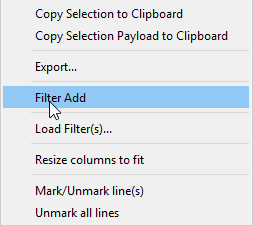
\includegraphics[width=0.3\textwidth]{images/rightmouse_tableview.png}
\end{figure}

\end{enumerate}


%~~~~~~~~~~~~~~~~~~~~~~~~~~~~~~~~~~~~~~~~~~~~~~~~~~~~~~~~~~~~~~~~~~~~~~~~~~~~~~~~~~~~~~~

\subsubsection{Viewer Configuration File}

The basic viewer configuration file is "config.ini". It e.g. stores the Viewer Settings, plugin states as well as size and windows position.
Its default location is:

\begin{verbatim}
~/.dlt/config ( on Linux )

and

C:\Users\<username>\.dlt\config ( on Windows )
\end{verbatim}


%C:\Users\\textless username\textgreater \.dlt\config ( on Windows 7 )

This file is not overwritten in case you reinstall the Viewer.
In case you install a new release of the viewer it may be better
to delete the file to avoid inconsistency.
A new instance of the file containing default values will be created when the viewer starts.


\pagebreak

%##################################################################################################
\section{Plugins}
\label{plugins}

The feature set of the DLT Viewer can be easily extended with DLT Viewer plugins.
Plugins have full read access to trace messages. They can decode messages,
provide additional representations inside the DLT Viewer GUI, control the Viewer or send injection messages
to target applications, depending on which DLT interfaces the respective plugin implements.
It is easy to write your own DLT Viewer plugin, examples are provided in the DLT Viewer source code.

Here is an overview of the some useful plugins:

%~~~~~~~~~~~~~~~~~~~~~~~~~~~~~~~~~~~~~~~~~~~~~~~~~~~~~~~~~~~~~~~~~~~~~~~~~~~~~~~~~~~~~~~~~~~~~~~~~~
\subsection{Non Verbose Mode Plugin}

\label{nonverbosemode}
Interface:
\begin{itemize}
    \item QDLTPluginInterface
    \item QDLTPluginDecoderInterface
\end{itemize}
Description:
    Decodes the DLT non-verbose messages after a catalog file has been loaded.


If you receive DLT messages in non verbose mode, you need to decode them
to see their plain text. To do this, go to the "Plugin" tab in the "Project" panel.
Double click on the plugin "Non Verbose Mode Plugin". In the dialog that appears,
you can open a configuration file to load. Use this to load a non verbose XML description file,
which corresponds to your software on the ECU. Hit "OK" and the Plugin shows a list of all available
non verbose messages. As soon as you select a DLT message you can view the
decoded information. Incoming messages that fit the description file will now get decoded. To also
decode the already received messages, hit "Apply Configuration" on the top of the "Plugin" tab.
This plugin has no visible widget.


\vspace{10mm}
Raw nonverbose messages example:\linebreak

\vspace{3mm}

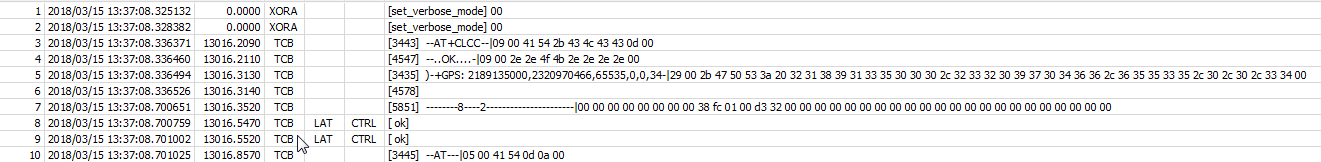
\includegraphics[width=1.0\textwidth]{images/nonverbose_raw.png}

Decoded nonverbose messages example:\linebreak

\vspace{3mm}

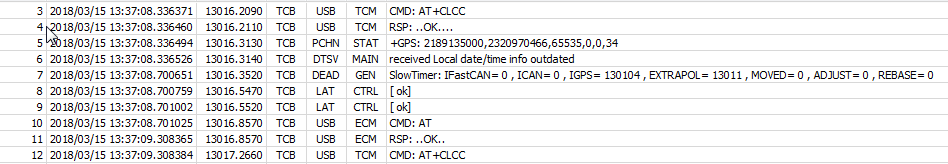
\includegraphics[width=0.8\textwidth]{images/nonverbose_decoded.png}

\subsubsection{DLT Parser}
To create an input file for this plugin based on your target DLT Daemon configuration in nonverbose mode, have a look on the tool
"DLT Parser". Also see the DLT Daemon documentation on the non verbose mode.

\begin{figure}[H]
 \centering
 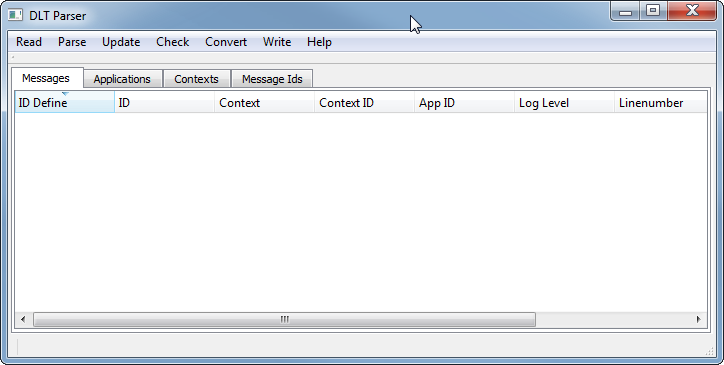
\includegraphics[width=0.6\textwidth]{images/dlt_parser.png}
 \caption{DLT Parser}
 \label{fig:dltparser}
\end{figure}




%~~~~~~~~~~~~~~~~~~~~~~~~~~~~~~~~~~~~~~~~~~~~~~~~~~~~~~~~~~~~~~~~~~~~~~~~~~~~~~~~~~~~~~~~~~~~~~~~~~
\subsection{DLT Viewer Plugin}

Interface:
\begin{itemize}
   \item  QDLTPluginInterface
   \item  QDLTPluginViewerInterface
\end{itemize}

Description:
    Advanced visual representation for selected log messages.
\linebreak

\begin{figure}[H]
 \centering
 \includegraphics[width=0.6\textwidth]{images/viewer_plugin.png}
 \caption{DLT Viewer Plugin widget}
 \label{fig:viewerpluginwidget}
\end{figure}

%\pagebreak

%~~~~~~~~~~~~~~~~~~~~~~~~~~~~~~~~~~~~~~~~~~~~~~~~~~~~~~~~~~~~~~~~~~~~~~~~~~~~~~~~~~~~~~~~~~~~~~~~~~
\subsection{DLT DBus Plugin}

Interface:
\begin{itemize}
    \item QDLTPluginInterface
    \item QDLTPluginViewerInterface
    \item QDLTPluginControlInterface
    \item QDLTPluginDecoderInterface
\end{itemize}
Description:\linebreak

Decode and show DBus messages.\linebreak

This is an example of raw DBus messages in the table view:\linebreak

\vspace{3mm}

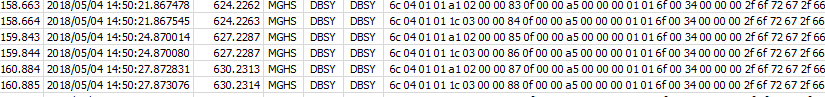
\includegraphics[width=0.8\textwidth]{images/dbus_table_raw.png}

\vspace{3mm}
This is how it looks like when the messages are decoded:\linebreak

\vspace{2mm}

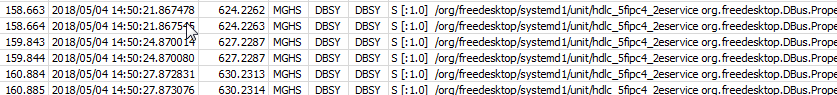
\includegraphics[width=0.8\textwidth]{images/dbus_table_decode.png}

\vspace{2mm}

In the plugin widget you get more detailed information about the DBus message.
And a more structured depiction in the Header tab.


\begin{figure}[H]
 \centering
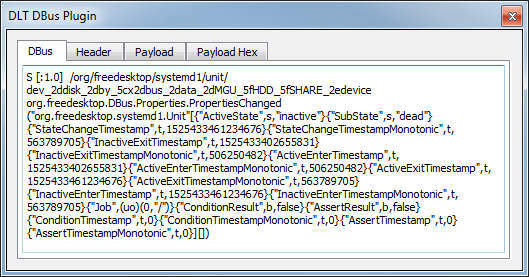
\includegraphics[width=0.6\textwidth]{images/dbus_widget.png}
 \caption{DLT DBus Plugin widget}
 \label{fig:dbuspluginwidget}
\end{figure}


\begin{figure}[H]
 \centering
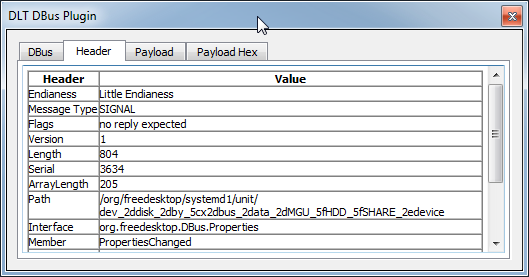
\includegraphics[width=0.6\textwidth]{images/dbus_widget_header.png}
 \caption{DLT DBus Plugin widget, Header tab}
 \label{fig:dbuspluginwidgetheader}
\end{figure}

\subsubsection{Configuration file}

DBUS messages are identified by a special combination of Apid/Ctid: the default is DBUS/ALL so in this case you do not load a special configuration file.\linebreak
But if you need other combinations of Apid/Ctid you need to specify this in the confuigration file.

Example: in case you need to use the two combinations of Apid/Ctid:

DBSY/DBSY

DBCN/DBCN


you have to enable these two combinations use the delivered example file \begin{verbatim}"dbusplugin_configuration.xml" \end{verbatim}
which is located in the plugins/examples folder (Windows) or /usr/share/doc/genivi-dlt-viewer (Ubuntu) of your viewer installation.
If the Apid/Ctids changes you can edit the file and change or add items for your need. The total amount of Apid/Ctid combinations
is limited to 10 due to performance reasons.\linebreak
The configuration file is loaded e.g. in the plugin configuration widget:


\begin{figure}[H]
 \centering
 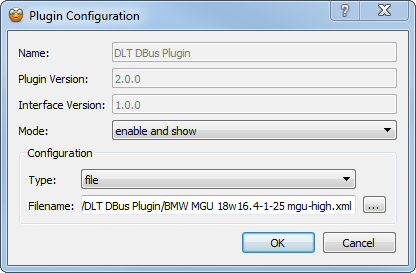
\includegraphics[width=0.6\textwidth]{images/dbus_configure.png}
 \caption{DLT DBus Plugin configuration widget}
 \label{fig:dbuspluginconfigurationwidget}
\end{figure}

%~~~~~~~~~~~~~~~~~~~~~~~~~~~~~~~~~~~~~~~~~~~~~~~~~~~~~~~~~~~~~~~~~~~~~~~~~~~~~~~~~~~~~~~~~~~~~~~~~~
\subsection{Filetransfer Plugin}

Interface:
\begin{itemize}
    \item QDLTPluginInterface
    \item QDLTPluginViewerInterface
    \item QDLTPluginControlInterface
\end{itemize}
Description:
    In case your log contains files like screenshots, coredumps etc. logged by a DLT Filetransfer application
    the objects can be viewed and saved with this plugin. \linebreak

\par

\begin{figure}[H]
 \centering
 %\includegraphics[width=0.6\textwidth]{images/filetransfer_plugin.png}
 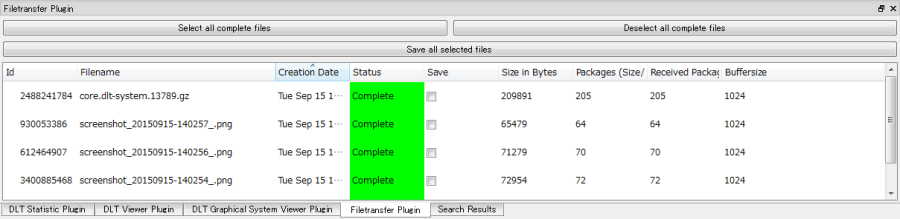
\includegraphics[width=1.0\textwidth]{images/filetransfer_list.png}
 \caption{File transfer widget}
 \label{fig:filetransferwidget}
\end{figure}


By double clicking the file name, you can see the file contents as preview and a text or image viewer is opened.

After enabling the filetransfer plugin when a dlt file already was loaded you will have to reload the logfile !

You can also use the Filetransfer Plugin command line mode to extract files out of a stored dlt file e.g. in an automated test setup.
On more information about the command line mode see \autoref{commandlinemode}.

\subsubsection{Configuration file}
In the subdirectory plugins/examples you find an example configuration file called \begin{verbatim}"filetransferplugin_configuration.xml"\end{verbatim}.
In case the target uses the default values to indicate file transfers you do not need to change anything here.
The default file transfer will work without additional configuration.

\subsubsection{Autosave feature}
In case you want to save transfered files automatically to a dedicated directory you can use the configuration file to
enable this feature by adding e.g.:

\begin{verbatim}
<?xml version="1.0" encoding="UTF-8"?>
<filetransferplugin_configuration>
<AUTOSAVE>c:/filetransfer/autosave</AUTOSAVE>   
</filetransferplugin_configuration>
\end{verbatim}

Every successfully completed file transfer will be stored to the given directory eg.g during live tracing but also when loading 
a dlt logfile.

The feature is enabled in filetransfer plugin starting from version 1.4.0.
%~~~~~~~~~~~~~~~~~~~~~~~~~~~~~~~~~~~~~~~~~~~~~~~~~~~~~~~~~~~~~~~~~~~~~~~~~~~~~~~~~~~~~~~~~~~~~~~~~~
\subsection{Plugin SDK}

More information about the Plugin SDK can be found in the seperate document dlt\_viewer\_plugins\_programming\_guide.pdf.
In the source code you also find four dummy plugins, ready to build. You can just use it as a template.

There are
\begin{itemize}
    \item dummycontrolplugin
    \item dummyviewerplugin
    \item dummycommandplugin
    \item dummydecoderplugin
\end{itemize}

%~~~~~~~~~~~~~~~~~~~~~~~~~~~~~~~~~~~~~~~~~~~~~~~~~~~~~~~~~~~~~~~~~~~~~~~~~~~~~~~~~~~~~~~~~~~~~~~~~~
\subsection{Using the plugins autoload feature}
\label{usingautoload}
For the nonverbose mode or the DBus plugin, the used configuration file may e.g. depend on the SW version of your target.
In case the DLT Daemon is configured to send out the target software version instead of the DLT Daemon version ( see DLT Daemon documentation )
you can automatically load the according configuration file needed by the plugin.\\
This is especially helpful if you work with traces of different ECUs or software versions.

See also \autoref{versionstring} for information about the version string.\\

To use the autolaod feature you need to create a subdirectory whichs name equals exactly the name of the choosen plugin, e.g.
"DLT DBus Plugin". In this directory you can place plugin configuration files whichs names exactly equal
the version string send by your target. So if you process logs with different target software versions
the correct configuration is automatically loaded accordingly.

\subsubsection{Plugin autoload example}

\begin{enumerate}
\item E.g. the  version string is "Aspire\_SW123":\linebreak
\vspace{0.2cm}

\includegraphics[width=0.2\textwidth]{images/versionstring_ecu.png}


\item Create a directory named "E:\textbackslash viewertests\textbackslash DLT DBus Plugin"
and place a configuration file namend "Aspire\_SW123.xml", ( or so named folder which contains this file ) there.\\

\vspace{0.2cm}
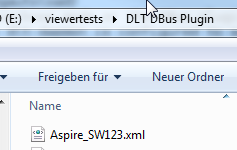
\includegraphics[width=0.4\textwidth]{images/autoloadexample_filename.png}

\item Set the plugins autoload path accordingly to "E:\textbackslash viewertests" and set the checkbox, see \autoref{enableautoload} \linebreak


\item Enable the plugin itself and load the dlt file or connect to the target

\item The configuration file is automatically processed as soon as the version string is received:

\vspace{0.3cm}

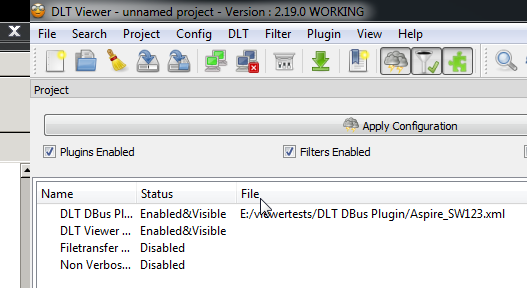
\includegraphics[width=0.4\textwidth]{images/pluginsautoloadprocessed.png}

\end{enumerate}

%~~~~~~~~~~~~~~~~~~~~~~~~~~~~~~~~~~~~~~~~~~~~~~~~~~~~~~~~~~~~~~~~~~~~~~~~~~~~~~~~~~~~~~~~~~~~~~~~~~
\subsection{Install, remove, enable and disable plugins}
\label{installremoveplugins}

\subsubsection{Windows}
The DLT Viewer will look for plugins in two places. The first place is the
"plugins" folder inside the main application path. After that, if a plugins path is
defined in the DLT Viewer settings ( see \autoref{pluginspath} ), the application will also look in this specified location for plugins.

You can install plugins by putting them into one of the directories mentioned,
and uninstall them by removing them from these directories.

It also is possible to enable or disable plugins in the DLT Viewer itself.
To do this, double-click or right-click on a plugin in the "Plugins" tab. You will get a
drop-down menu for enabling and disabling the plugin. When enabled,
messages are passed to the plugin. When disabled, the plugin will be ignored in
the message processing chain. For plugins that implement the "viewer" interface,
there is also a third selection, "Enable and Show", which brings up the UI widget of
this plugin.

\subsubsection{Linux}


On Linux, organizing plugins works in a similar fashion. In addition to the previously mentioned folders,
the Linux version will also look into "/usr/share/dlt-Viewer/plugins" for any plugins.
You will need to have root permissions to modify the plugin directories that are installed system-wide.
To organize plugins without root permissions, you can set the user defined plugin directory in the DLT Viewer
settings to some other path, e.g. somewhere in your home directory.

%##############################################################################################


\section{Best Practices}

%~~~~~~~~~~~~~~~~~~~~~~~~~~~~~~~~~~~~~~~~~~~~~~~~~~~~~~~~~~~~~~~~~~~~~~~~~~~~~~~~~~~~~~~~~~~~~~~~~~
\subsection{Connect to ECU}
\label{connecttoecu}

Press the connect button \includegraphics[width=0.03\textwidth]{images/connect_button.png} to connect to the target:\linebreak

If no ECU is configured, the ECU configuration dialog appears.
Select the "Interface Type" you want to use (TCP, UDP or serial).
The ECU configuration dialog also can be envoked by selecting right mouse button "ECU add"
in the Project Config Panel.

\begin{figure}[H]
 \centering
 %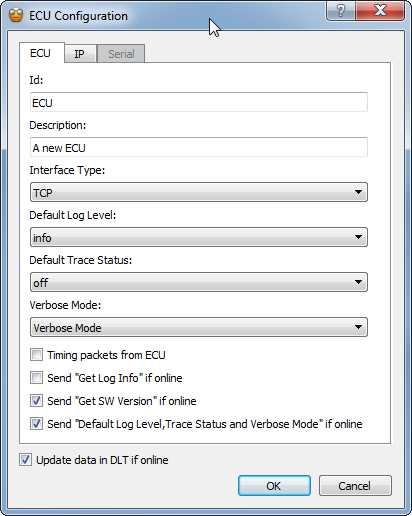
\includegraphics[width=0.6\textwidth]{images/ecu_dialog_2_19_0.png}
 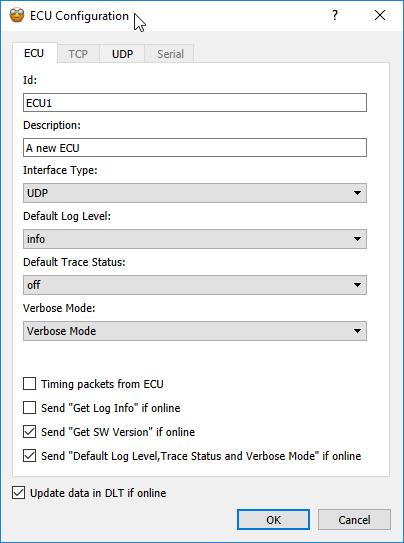
\includegraphics[width=0.6\textwidth]{images/ECU_dialog.png}
 \caption{ECU dialog}
 \label{fig:ecudialog}
\end{figure}



Here you can set some basic parameters like

\begin{itemize}
 \item Id\linebreak Identifier of the "Electronic Control Unit" used in the config tab. If it is left at its default value (ECU1) it will automatically be set by the ECU messages which come with the connection.
 \item Description\linebreak Description of the ECU Id used in the config tab
 \item Interface Type\linebreak You can choose TCP, UDP or Serial
 \item Default Log Level ( equals "Subtype" in the message table ), see also \autoref{loglevels}
 \item Default Trace Status ( on / off )
 \item Verbose Mode ( yes / no )\linebreak See also \autoref{nonverbosemode}
 \item Timing packets from ECU\linebreak Request the ECU to send additional timing messages ( see daemon documentation )
 \item Send "Get Log Info" if online\linebreak See \autoref{getallcontexts}
 \item Send "Get SW Version" if online\linebreak Request SW version from daemon, see also \autoref{versionstring}
 \item Send "Default Log Level,Trace Status and Verbose Mode" if online
 \item Update data in DLT if online\linebreak Send the above selected request to the ECU always when connecting to it
\end{itemize}

%~~~~~~~~~~~~~~~~~~~~~~~~~~~~~~~~~~~~~~~~~~~~~~~~~~~~~~~~~~~~~~~~~~~~~~~~~~~~~~~~~~~~~~~~~~~~~~
\subsubsection{TCP}

If you choose a TCP connection enter the the hostname or the IP address.\linebreak
Format is e.g.192.168.0.5 of the target ECU.
\linebreak
In case of an IPv6 address just use the format ( e.g. ) fe80::xxxx:xxxx:xxxx:\%eth1


IPv4 example:

\begin{figure}[h]
 \centering
 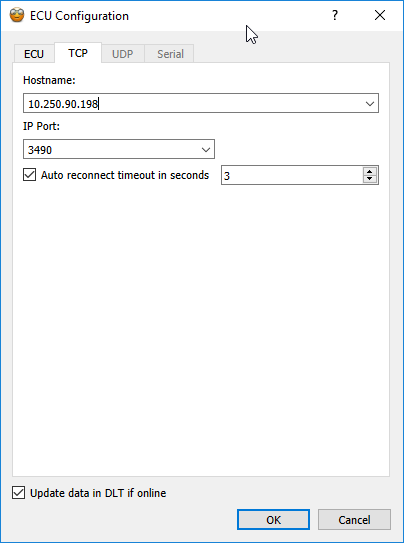
\includegraphics[width=0.6\textwidth]{images/tcp_applet01.png}
 \caption{IP configuration tab}
 \label{fig:ipconfigurationtab}
\end{figure}


%~~~~~~~~~~~~~~~~~~~~~~~~~~~~~~~~~~~~~~~~~~~~~~~~~~~~~~~~~~~~~~~~~~~~~~~~~~~~~~~~~~~~~~~~~~~~~~
\subsubsection{UDP}

In case of UDP reception you are able to specify the interface and the IP port where you expect the 
UDP datagrams to be received. The selection box "Receiving interface" will offer you all available 
ethernet interfaces of your machine. In case of AnyIP the oprating system will choose an interface for you.
To receive multicast messages you can activate "Multicast on network interface" and specify the UDP multicast address
to join the multicast group accordingly.

\caution{On Windows machines it was observed that the selection of the specific IF instead of AnyIP is essential}

IPv4 example:

\begin{figure}[h]
 \centering
 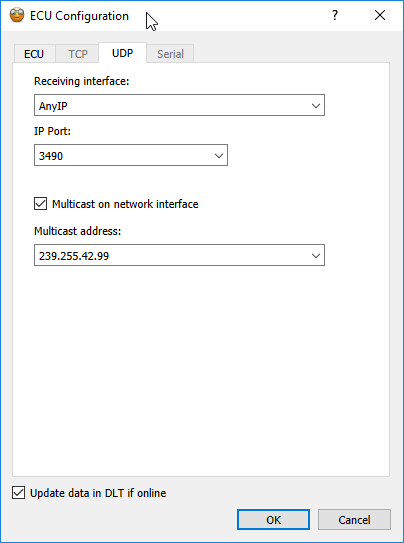
\includegraphics[width=0.6\textwidth]{images/ECU_dialogUDP.png}
 \caption{UDP configuration tab}
 \label{fig:udpconfigurationtab}
\end{figure}



%~~~~~~~~~~~~~~~~~~~~~~~~~~~~~~~~~~~~~~~~~~~~~~~~~~~~~~~~~~~~~~~~~~~~~~~~~~~~~~~~~~~~~~~~~~~~~~
\subsubsection{Serial}


If you choose a serial connection, select the serial port here. Check the COM port
where your serial device is connected to in your Windows configuration. A drop down
list provides a list of examples for the port configuration.

\begin{figure}[H]
 \centering
  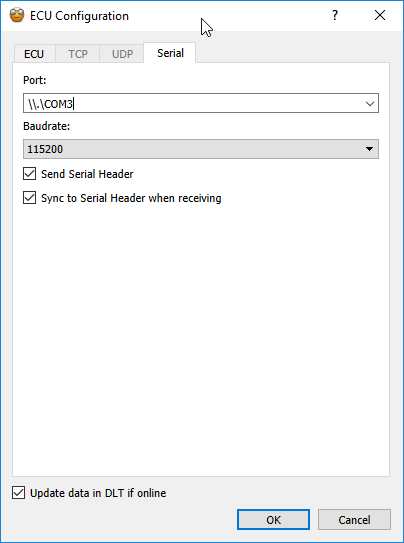
\includegraphics[width=0.6\textwidth]{images/ecu_dialog_serial01.png}
 \caption{Serial configuration tab}
 \label{fig:serialconfigurationtab}
\end{figure}

If you select "OK" the DLT Viewer will try to connect to the ECU.
The ECU Id shows "online" (green) as soon as the DLT Viewer is connected to the
specified device.
All received DLT messages should then be displayed in DLT message table.

\pagebreak

%~~~~~~~~~~~~~~~~~~~~~~~~~~~~~~~~~~~~~~~~~~~~~~~~~~~~~~~~~~~~~~~~~~~~~~~~~~~~~~~~~~~~~~~~~~~~~~
\subsection{Available List of Applications and Contexts}


\subsubsection{Hierarchy}

Applications and contexts are organized in a hierarchy. Each ECU connection can have
several applications. Each application can have several contexts. Contexts are the instance
where the loging application configures log levels and trace status.

In the Project/Config tab you will see a tree with all used applications and contexts in a sub
tree of an ECU.

\subsubsection{Get all used contexts from ECU}

\label{getallcontexts}
In case you are connected to the ECU you can get all used contexts by double click on the
ECU item in the Project/Config tab and select menu item "DLT Get log info".
The DLT Viewer then sends a request to the target and receives a response message
with all available contexts and their log levels. The list of available contexts is added
to your "Config" list.

\begin{figure}[H]
 \centering
  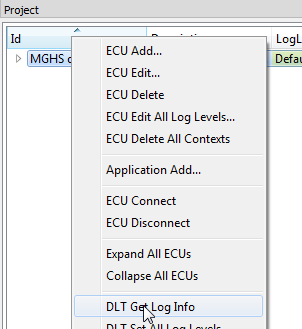
\includegraphics[width=0.4\textwidth]{images/getloginfo.png}
 \caption{Get log info}
 \label{fig:getloginfo}
\end{figure}


\subsubsection{Automatically update used context}

There are several possibilities how to automatically update the list of contexts of a ECU.

%\subsubsubsection{Get context list when connected to ECU}
\paragraph{Get context list when connected to ECU}

Each time you connect to the ECU you can get a list of all used context.
You can activate this feature in the ECU configuration by activating "Send Get Log Info if
online". See \autoref{fig:ecudialog}.

\paragraph{ECU sends automatically new registered contexts}

This feature must be activated in the DLT daemon configuration of the ECU.

\pagebreak

%~~~~~~~~~~~~~~~~~~~~~~~~~~~~~~~~~~~~~~~~~~~~~~~~~~~~~~~~~~~~~~~~~~~~~~~~~~~~~~~~~~~~~~~~~~~~~~

\subsection{Log levels and trace status configuration}

\label{loglevels}
Each DLT log message provides a log level. The following table shows the different available
log levels and describes in which use cases they should be used.


%\begin{longtable}{| l | m{3cm}  | m{11cm} |}
\begin{longtable}{| l | m{11cm}  | m{11cm} |}
\caption[GUI section description]{GUI section description} \label{guisectiondescription} \\
 \hline
   \textbf{Log Level} & \textbf{Usage} \\
\hline
%1 Zeile
   DLT\_LOG\_FATAL
   &
   Fatal errors are errors which prevents the software to continue working. \\
   \hline
%2 Zeile
   DLT\_LOG\_ERROR
   &
   Normal errors are errors which are detected by the software, but do not
   prevent the software to continue working. \\
   \hline
%3 Zeile   
   DLT\_LOG\_WARN
   &
   Warnings are used when some minor problems are detected. 
   \\
%4 Zeile    
   \hline
    DLT\_LOG\_INFO
   &
   Info is the standard log level. It is used to display all kind of
   information, so that the device tester knows that the functionality of the
   software is correctly working. This log contains e.g. version
   information or state change information of SW modules. \\
%5 Zeile   
   \hline
   DLT\_LOG\_DEBUG 
   &
   This log level is normally turned off. It should be used to
   display some more deep information about the functionality of a
   software component. \\
%6 Zeile   
   \hline
   DLT\_LOG\_VERBOSE
   &
   This log level is normally turned off. This log level provides huge
   amount of logs from a SW component and should only be
   enabled for individual SW components. \\
   \hline

\end{longtable}


In case the default log level is set to DLT\_LOG\_INFO for the ECU, all log messages from
DLT\_LOG\_FATAL to DLT\_LOG\_INFO are send out by the daemon and displayed. 

DLT\_LOG\_DEBUG and DLT\_LOG\_VERBOSE messages are not generated in this use case.


\subsubsection{Get default log level}

Request the current default log level directly from the ECU.

\subsubsection{Set ECU default log level}

The default log level can be set for each ECU connection separately. Just open a current ECU
configuration by double click on the ECU item in the Project/Config tab.
You can change the value of "Default Log Level" and "Default Trace Status" and press OK.
If you are connected the new default values are send to the ECU immediately. All Contexts
which are set to "default" get the new default values. The option "Update data in DLT if online"
must be activated.
When you connect to the ECU the configured default values are send immediately.
See \autoref{fig:ecudialog}.

\subsubsection{Edit all log levels}

Here you can edit and set the loglevels for all contexts at once.
If the checkbox "Update data in DLT if online" then the log level for all contexts is set.
E.g. you can switch off tracing for all log levels at once. In this case the DLT daemen does not send out
any messages except DLT control messages.


\subsubsection{Set individual log levels}

To set individual log levels and trace status for a dedicated context you can to double click on the context item in the
"Project/Config" tab. A Context configuration dialog is opened where you can set individual
log level and trace status. Press Ok to send the changed log level to the ECU.

\begin{figure}[H]
 \centering
  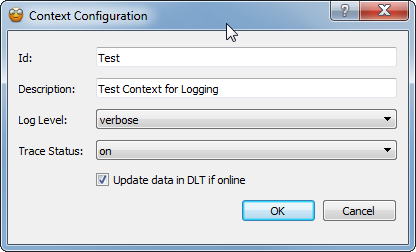
\includegraphics[width=0.4\textwidth]{images/contextconfiguration.png}
 \caption{Context configuration}
 \label{fig:contextconfiguration}
\end{figure}


\subsubsection{Set all configured log levels of all contexts}

You can send all configured log levels, e.g. when you stored the log levels in the project file.
Right click on a ECU item in the "Project/Config" tab and press the menu item "DLT Set All Log levels":

\begin{figure}[H]
 \centering
  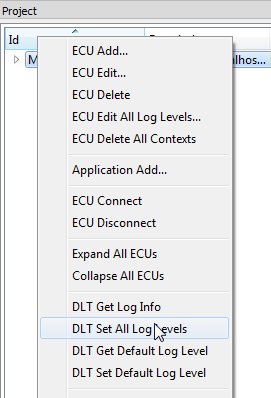
\includegraphics[width=0.4\textwidth]{images/setallloglevels.png}
 \caption{DLT Set all loglevels}
 \label{fig:setallloglevels}
\end{figure}


\subsubsection{Store all log levels and trace status in ECU}

You can store the current configuration of all log levels on the ECU. After restart of the ECU
the current set log levels and trace status are available again.
Right click on a ECU item in the "Project/Config" tab and press the menu item "Store Config":

\begin{figure}[H]
 \centering
  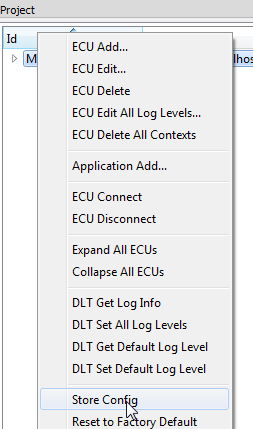
\includegraphics[width=0.3\textwidth]{images/storeloglevel.png}
 \caption{Store all loglevels}
 \label{fig:storeloglevels}
\end{figure}

\pagebreak
%~~~~~~~~~~~~~~~~~~~~~~~~~~~~~~~~~~~~~~~~~~~~~~~~~~~~~~~~~~~~~~~~~~~~~~~~~~~~~~~~~~~~~~~~~~~~~~
\subsection{Status line information}

In the GIU status line you find sveral additional information

\subsubsection{Logfile location}


\subsubsection{The version string}
\label{versionstring}
Depending on the setting "ECU Software version info" in dlt.conf configuration of the DLT Daemon
the daemon sends either the daemon version or the content of a given file on the target periodically.
The version is transmitted by a special control message, for example:

Header detected after end of message, offset: 14
ERROR in file detected at index 0 msg length 71 file position 42

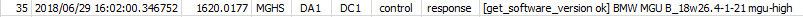
\includegraphics[width=1.0\textwidth]{images/versionstring_message.png}

You also can request the version string manually:

Right click on a ECU item in the "Project/Config" tab and press the menu item "Get software version".


The version string is shown in the status line (see \autoref{footer}) of the dlt viewer.
%when configured in "PathToECUSoftwareVersion".
Assumend this method is used to identify target and software version you can also use it for plugins
autoload feature, see also \autoref{usingautoload}.\linebreak

Version string example 1 ( daemon version )\linebreak

\vspace{0.3cm}

\includegraphics[width=0.6\textwidth]{images/versionstring_daemon.png}

\vspace{0.5cm}

Version string example 2 ( daemon version with tooltip )\linebreak

In case the version string is too long to be displayed in the status line you can see the full name in the tooltip by hoovering above the version string.\\

\vspace{0.2cm}

\includegraphics[width=1.0\textwidth]{images/versionstringwithtooltip.png}

\subsubsection{File errors}
Shows the amount of detected errors when loading a dlt logfile. In commandline mode
you get more detailed information in case file error was detected. E.g.:

 

\subsubsection{Receive counter}
In live tracing mode the tab "Recv:" shows the amount of currently received data in messages

\subsubsection{Receive error counter}
In live tracing mode the tab "Recv Errors:" shows the number of envcountered receive errors

\subsubsection{Sync found}
In serial connection mode this counter shows ...


\pagebreak
%~~~~~~~~~~~~~~~~~~~~~~~~~~~~~~~~~~~~~~~~~~~~~~~~~~~~~~~~~~~~~~~~~~~~~~~~~~~~~~~~~~~~~~~~~~~~~~

\subsection{Working with DLT Log Files}
When you start the DLT Viewer, a temporary log file is created. The default location of these logfiles is configurable (see \autoref{temporaryfile}) in the Global Settings Tab.
All received DLT messages get stored in this temporary log file and shown in the DLT message table.
A file containing messages usually is associated with a target / ECU connection. In case of livetracing the messages received from all connected
ECUs are stored in the same file.
%\vspace{5cm}

\subsubsection{Save as}
Select the menu option "File"\ensuremath{\rightarrow}"Save as" or \includegraphics[width=0.03\textwidth]{images/saveas_icon.png} to save a file.
Saving a file just renames the current tmp file and stores it to the selected destination, the received messages are still
added to this file and the file is processed / accessed by the DLT Viewer. A saved file also contains information about ECU configuration, Apids, Ctids
and log levels.

\caution{In case you did open multiple files to concatenate them, e.g. by Drag\&Drop then only the last opened file will be saved. If you want to save all files in one please use "Export ..."}

\subsubsection{Export}
Select the menu option "File"\ensuremath{\rightarrow}"Export... ". 
There are several options for exporting messages:
\vspace{0.3cm}

\begin{figure}[H]
 \centering
   \includegraphics[width=0.5\textwidth]{images/DLTExporter.png}
 \caption{Exporter dialog}
 \label{fig:exportdialog}
\end{figure}


\begin{enumerate}
\item Format: file format of the exported messages
  \begin{enumerate}
   \item DLT: DLT binary format, the file can be loaded and processed by DLT Viewer.
   \item DLT Decoded: store the selection in DLT binary format, the resulting file can be loaded and processed
       by DLT Viewer. In case a decoder plugin was active, the decoded message payload is stored in human readable way.
   \item UTF8: stores the selection as UTF8 text file.
   \item ASCII: stores the selection as ASCII text file.
   \item CSV: like ASCII but columns are seperated by semicolon.
 \end{enumerate}
 \item Selection: choose which messages to be exported
  \begin{enumerate}
   \item All: all messages in the current logfile.
   \item Filtered: only messages which apply to the active filters.
   \item Marked: all marked lines are exported. Marked lines are either manually marked in the table view or lines marked by a filter.
        "Automarked" lines like warn/error or marker messages are not taken into account.
  \end{enumerate}
\end{enumerate}

\subsubsection{New file or open file}
Select the menu option "File"\ensuremath{\rightarrow}"New/Open" to create a new or open an existing log file.

\subsubsection{Import DLT Stream}
Select the menu option "File"\ensuremath{\rightarrow}"Import DLT Stream" to import a an existing log file
which does not contain DLT file storage headers.
The logfile messages are imported into the currently opened dlt file.

\subsubsection{Import DLT Stream Serial}
Select the menu option "File"\ensuremath{\rightarrow}"Import DLT Stream" to import an exiting serial log file.
Just the logfile messages are imported without an ECU configuration or Apid / Ctid informations.

\subsubsection{Append DLT File}
Select the menu option "File"\ensuremath{\rightarrow}"Append DLT File" to append the message content of the
selected file to a current file.
The message index is automatically increased but the messages may not be in the correct order regarding reception time stamp.
This can be achieved by "Filters Enabled" with "Sorted by Time". See \autoref{sortbytime}.

\subsubsection{File clear}
Select "File"\ensuremath{\rightarrow}"Clear" or \includegraphics[width=0.02\textwidth]{images/clean_icon.png}
to clear the current log file. The message table view and the indexes as well as the search result windows are cleared.
If configured, a new tmp file is automatically opened.

\subsubsection{Open multiple files}

Data logging devices usually create logfiles of a determined size. So for analyzing a trace you may need to concatenate
these files to one single file. On a Linux machine you e.g. could do that with:\linebreak "cat *.dlt >> resulting.dlt"\linebreak
cat *.dlt accesses the files sorted by the file name, that means the correct order of the file must be determined
by the file name.

\begin{comment}
This is what drag and drop of the dlt viewer does. Usually you can not rely on the time stamp of the files because some
copy mecchnism or other file processing may alter the files time stamp

RAUSFINDEN  wie das funnktioniert: creation time stamp und access time stamp

3 Files erzeugen und touchen, dann öffnen und drag&drop ...
\end{comment}

\subsubsection{Searching and navigating in the logfile}
\paragraph{Jump to line / index}
Select Menu "Search"\ensuremath{\rightarrow}"Jump to" or keypress combination "STRG + G" to directly navigate to the desired line / index number in the table view.

\paragraph{Quicksearch}
Using the input field in the menu bar you can perform a quicksearch, the string entered is used a search pattern to find matches in the payload of all messages as configured in the Search Dialog. Use the 
green arrows \includegraphics[width=0.06\textwidth]{images/green_arrows.png} in the menu bar to navigate in single step mode or fill the search results window.

\paragraph{Advanced search}
If you want to specify more details and other search parameters you can use the Menu "Search"\ensuremath{\rightarrow}"Find" or
search icon \includegraphics[width=0.03\textwidth]{images/searchicon.png} in the toolbar to open the search dialog.

\begin{figure}[H]
 \centering
  \includegraphics[width=0.5\textwidth]{images/Search.png}
 \caption{Search dialog}
 \label{fig:searchdialog}
\end{figure}


\begin{itemize}
 \item Text to search\linebreak The search string you are looking for in the trace.
 \item Search from:\linebreak Search whole log or starting from the current selected line.
 \item Highlight color:\linebreak Select the color to highlight the hit line in single step mode.
 \item Find all:\linebreak If enabled then all search hits are listed in the search results window, else the search runs in single step mode:
 jump to the results with Previous ( F2 ) or Next ( F3 ) or  using the green arrows \includegraphics[width=0.06\textwidth]{images/green_arrows.png} in the menu bar.
 \item Search in Header\linebreak Search hits in the message header will be shown too. E.g. search for a certain receive or target time stamp.
 \item Search in Payload\linebreak Search hits in the message payload will be displayed. This is most probably the standard option.
 \item Search Options: Case Sensitive\linebreak \caution{If enabled the search time may increase significantly !}
 \item Search Options: Regular Expression\linebreak Use regular expression search.
 \item ApId\linebreak Only take care of messages with this ApId.
 \item CtId\linebreak Only take care of messages with this CtId.
 \item Timestamp start / end\linebreak All search hits will have target time stamps within the given time range will be shown.
 \item Payload start / end\linebreak All search hits will be in the range of a payload which contains the given start
     string and a payload which contains the given stop string will be shown.
\end{itemize}


\paragraph{Search history}
You can use the menu "Search"\ensuremath{\rightarrow}"History" to select the last used search strings.
There also is a drop - down menu in the search input field of the toolbar to select the last used search strings.


\subsubsection{Setting a Marker}

\label{settingmarker}
When you set a marker in the logfile using DLT \ensuremath{\rightarrow} Marker, or just click on the icon: \includegraphics[width=0.02\textwidth]{images/marker_icon.png},
a marker line is added to the bottom of the current trace, this is especially meaningfull when live tracing
to mark a certain point in the log.\linebreak

The marker line looks like this:\linebreak

% \begin{verbatim} 1 2018/06/26 14:51:05.000000 24878.2430 0 DLTV DLTV DLTV 0 control response non-verbose 0 MARKER \end{verbatim}
\includegraphics[width=1.0\textwidth]{images/markermessage.png}

These marker messages can be automatically highlighted in green color, see in \autoref{automarkmarker} in Settings / Project Other.

But keep in mind: Marker messages are "control messages". So they are not displayed in case "Write Control Messages to log file" is not enabled.
See \autoref{controlmessagestolog} in Settings / Project Other.

%\caution{You will NOT see the marker messages in case "Write Control Messages to log file" is not enabled}

%~~~~~~~~~~~~~~~~~~~~~~~~~~~~~~~~~~~~~~~~~~~~~~~~~~~~~~~~~~~~~~~~~~~~~~~~~~~~~~~~~~~~~~~~~~~~~~
\subsubsection{Logging only mode}
\label{Loggingonlymode}
In case you only want to record traces for later analysis without viewing them in the DLT message table,
it is recommended to enable the "Logging only mode". All plugins and the main table view are disabled.
So you reduce performance impact and the probability of a viewer crash e.g. due to a faulty plugin.

See \autoref{enableloggingonlymode}, "Viewer Configuration Settings/Project Other", how to enable it.

Basically you also can use the commandline tool dlt-receive to receive dlt messages and write them to a file.
It is part of the dlt-daemon and so only is available on Linux systems.

Example:

\begin{verbatim}
dlt-receive -o ./logit.dlt 160.48.199.99
\end{verbatim}



\pagebreak

%~~~~~~~~~~~~~~~~~~~~~~~~~~~~~~~~~~~~~~~~~~~~~~~~~~~~~~~~~~~~~~~~~~~~~~~~~~~~~~~~~~~~~~~~~~~~~~
\subsection{Working with Filters}
\label{workingwithfilters}


\subsubsection{Sort by Time}
\label{sortbytime}
If the filters are enabled, even if there is no active filter applied, you can select "Sorted by Time" in the
Filter tab of the Project Panel. In this case all messages will be sorted by received time.

E.g. in case you load several logfiles which contain messages from different ECUs you will get the messages sorted by the recveive time instead by the message index.

\caution{Take care of the (target) Timestamp - it may happen that messages are not received in the order
like they are emitted by the specific application on the target but like they are sent out by the target system}

\subsubsection{Sort by Timestamp}
\label{sortbytimestamp}
You can select either "Sorted by Time" or "Sorted by Timestamp" in the
Filter tab of the Project Panel. In this case all messages will be sorted by the timestamp the messages get when issued
by the sending application on the target. 

\caution{When sorting by (target) timestamp be sure that the trace contains messages of one lifecycle only, otherwise you will mix them up with
several timestamps from different lifecycles which might be confusing}



\subsubsection{How to create a filter}

You can find some example filters in your viewer installation directories and in the source code in directory "filters":
\begin{verbatim}
 * control_messages.dlf
 * error_fatal_messages.dlf
 * message_buffer_overflow.dlf
 * software_version.dlf
\end{verbatim}

In case you define filters please take into account that message filtering has performance impact. It is recommended to combine sevaral search parameters in one filter definition instead of cascading multiple filters.
When searching for payload content you can improve performance if you also limit the filter using a certain Ctid or Apid where you expect your message in.

\caution{More and complex filters slow down the viewer !}

There are several ways to add a filter:
\begin{enumerate}
\item Menu "Filter"\ensuremath{\rightarrow}"Filter Add"
\item On a context or application item in the Config tab of the Project Panel: selecting right mouse button "Filter Add".
The avaiable Ecuid, Apid, Ctid will be filled in already.
\item On a message in the message table view select a line and right mouse button "Filter Add". All message elements except log levels are filled in already.
\end{enumerate}


\label{createfilter}
\begin{figure}[H]
 \centering
  \includegraphics[width=0.6\textwidth]{images/Filter_Configuration.png}
 \caption{Filter configuration}
 \label{fig:filterconfiguration}
\end{figure}


\begin{enumerate}
\item Name: any name describing your filter function
\item Type: \linebreak
      Positive ( default): all hits which match the filter will be shown in the message table\linebreak
      Negative: messages which fit the filter will NOT be shown in the message table\linebreak
      Marker: messages which fit the filter will just be highlighted with the choosen color\linebreak
\item Marker color: choose a proposed color or create on from the color palette
\item ECU Id
\item Application Id
\item Context Id
\item Header Text: the string consist of all the message header data like Time, Timestamp, Ecuid ...
      ( regardless if displayed in the table view )
\item Payload Text
\item Log Level Min
\item Log Level Max
\item Control Messages
\end{enumerate}


\subsubsection{Using regular expressions}
You can create more complex filters by making use of the Qt regular expressions, e.g. using wildcards and so on.
To enable regular expressions select the checkboxes "regex" available for Ctid, Header Text and Payload Text.

\caution{Regular expressions allow complex and conditional search criteria but can slow down the filter performance tremendously}

\subsubsection{Recommendations and examples}

\paragraph{Filtering for multiple context IDs}
For filtering mutilple Ctids use one filter with "TC|HADT|PRER|GNRL" as a regular expression in "Context Id" instead of defining four seperate filters.

\paragraph{Filtering for message payload containing multiple strings}

E.g. in case you want to filter out all lines where the payload contains the strings "getBatterieData" or "message start" use:

\begin{verbatim}
(getBatterieData|message start)
\end{verbatim}

as "Payload Text" and enable RegExp in the filter configuration

\paragraph{Filtering for certain loglevel only}
If you only want to see messages between loglevels fatal and warn you should set Log Level Min to warn and Log Level Max to fatal


\pagebreak
%~~~~~~~~~~~~~~~~~~~~~~~~~~~~~~~~~~~~~~~~~~~~~~~~~~~~~~~~~~~~~~~~~~~~~~~~~~~~~~~~~~~~~~~~~~~~~~
\subsection{Project Files}
\label{projectfiles}
You can save project specific settings like the status of plugins ( including used configuration files ), active filters, ECU autoconnet and so on for later reuse
in a project file. The project file extension is "*.dlp".
The project file rules the standard configuration settings of config.ini.
You also can specify a project file as default to be automatically loaded at viewer start, see \autoref{defaultproject} in \autoref{globalsettings}.

Projectfiles can also be specified in a command line call and are especially helpful here.
Select Menu "Project" to manage project files. To save the current settings you also can press the "save project" icon \includegraphics[width=0.02\textwidth]{images/saveprojecticon.png}

\pagebreak
%~~~~~~~~~~~~~~~~~~~~~~~~~~~~~~~~~~~~~~~~~~~~~~~~~~~~~~~~~~~~~~~~~~~~~~~~~~~~~~~~~~~~~~~~~~~~~~
\subsection{Command line mode}
\label{commandlinemode}
If you call the DLT Viewer on command line you get the following output:

\subsubsection{Commandline help}

dlt\_viewer -h ( Linux ) or dlt\_viewer.exe -h ( Windows )

\footnotesize\begin{verbatim}
Usage: dlt_viewer [OPTIONS]
Options:
 -h Print usage
 -p projectfile          Loading project file on startup (must end with .dlp)
 -l logfile              Loading logfile on startup (must end with .dlt)
 -f filterfile           Loading filterfile on startup (must end with .dlf)
 -s or --silent          Enable silent mode without warning message boxes.
 -v or --version         Only show version and buildtime information
 -c logfile textfile     Convert logfile file to textfile (logfile must end with .dlt)
 -u Conversion will be done in UTF8 instead of ASCII
 -csv Conversion will be done in CSV format
 -d Conversion will NOT be done, save in dlt file format again instead
 -dd Conversion will NOT be done, save as decoded messages in dlt format
 -e "plugin|command|param1|..|param<n>"         Execute a plugin command with <n> parameters.

Examples:
  dlt_viewer -c ./traces/trace.dlt ./trace.txt
  dlt_viewer -s -c -u ./trace/trace.dlt ./trace.txt
  dlt_viewer -s -d -c ./trace/trace.dlt ./trace.dlt
  dlt_viewer -s -p ./proj/decodeded.dlp -dd -c ./trace/trace.dlt ./trace.dlt
  dlt_viewer -s -csv -c ./trace/trace.dlt ./trace.csv
  dlt_viewer -s -d -f ./filter/filter.dlf -c ./trace/trace.dlt ./filteredtrace.dlt
  dlt_viewer -p ./proj/export.dlp -l ./trace/trace.dlt -e "Filetransfer Plugin|export|./ftransferdir"
\end{verbatim}
\normalsize

\subsubsection{Command line run}
You can just start the viewer on command line to get more detailed output on console.
As on windows the console currently is closed when giving no parameter you have to use -s or
-l as a workaround. At the beginning you get information about DLT Viewer version, build date and plugin status.
Also you get some debug output on what the viewer actual is doing.

Example output:

\begin{verbatim}
C:\01-viewer\r690>dlt_viewer.exe -s
Enable silent mode
Start "dlt_viewer.exe"
Build time Jun 15 2018 09:24:40
Version 2.19.0 WORKING
**********************************************************
Loading plugin "DLT Viewer Plugin" "1.0.1"
Loading plugin "Filetransfer Plugin" "1.2.1"
Loading plugin "Lifecycle Plugin" "1.3.1"
Loading plugin "Non Verbose Mode Plugin" "1.0.0"
Activate plugin "DLT Viewer Plugin" 1.0.1
Try to connect to ECU "160.48.199.99" "12:55:43"
Reconnect timeout for "160.48.199.99"
...
\end{verbatim}

\subsubsection{Examples}



\par
Command line usage examples:


\paragraph{Extract files from logfile using the fileransfer plugin}

You can use the Filetransfer Plugin to extract files out of a stored dlt file e.g. in an automated test setup.
To do this, call the Viewer with this command and parameters:

dlt\_viewer.exe -p x.dlp -l y.dlt -e "Filetransfer Plugin{\textbar}export{\textbar}[path\_to\_extract]"


\begin{itemize}
    \item dlt\_viewer.exe:\linebreak
    The executable of the DLT Viewer. E.g. dlt\_viewer.exe in Windows, dlt\_viewer in Linux
    \item x.dlp:\linebreak
    A project settings file which has the filetransfer properly configured, e.g. by setting a valid plugin xml file ( if needed )
    \item y.dlt:\linebreak
    Path to a dlt trace file containing embedded files which shall be extracted
    \item -e:\linebreak
    triggers the plugin internal command ( depending on plugin implementation )
    \item "Filetransfer Plugin":\linebreak
    Filetransfer Plugin will be called for the command interface
    \item export:\linebreak
    the plugin internal function "export" is addressed
    \item {[path\_to\_extract]}:\linebreak
    Path to the folder where you want to extract all file dumps. If you apply this for a lot of files,
    think about using individual paths, to avoid overwriting files with identical names.
\end{itemize}


\paragraph{Command line start of GUI with dedicated logfile}
\begin{verbatim}
dlt_viewer -l ./example.dlt
\end{verbatim}

\paragraph{Command line start of GUI with dedicated logfile and filterfile}
\begin{verbatim}
dlt_viewer -l ./example.dlt -f ./filter.dlf
\end{verbatim}


\paragraph{Convert to ASCII file}
\begin{verbatim}
dlt_viewer -c ./example.dlt ./example.txt
\end{verbatim}

\paragraph{Convert to UTF8 file}
\begin{verbatim}
dlt_viewer -u -c ./example.dlt ./example.txt
\end{verbatim}


\paragraph{Convert to ASCII file in silent mode}
\begin{verbatim}
dlt_viewer -s -c ./example.dlt ./example.txt
\end{verbatim}

\paragraph{Filter and convert to ASCII file}
\begin{verbatim}
dlt_viewer -f /viewertests/filterfiles/export.dlf -c ./example.dlt ./example.txt
\end{verbatim}

\paragraph{Filter, decode and convert to ASCII file}
\begin{verbatim}
dlt_viewer -p /viewertests/filterfiles/example.dlp -c ./example.dlt ./example.txt
\end{verbatim}


\paragraph{Filter and save as DLT file}
\begin{verbatim}
dlt_viewer -s -d -f /filterfiles/filter.dlf -c ./example.dlt ./example_filtered.dlt
\end{verbatim}

\paragraph{Filter, decode and save as DLT file}
\begin{verbatim}
dlt_viewer -s -dd -f /project/example.dlp -c ./example.dlt ./example_decoded.dlt
\end{verbatim}

\paragraph{Decode and save as DLT file}
\begin{verbatim}
dlt_viewer -p ./export.dlp -l ./filetransfer.dlt -e "Filetransfer Plugin|export|./ft_dir"
\end{verbatim}

\subsubsection{Shell script examples of command line calls}

You also can place dlt viewer command line calls to be used in shell scripts for use
in automated logfile processing, e.g. in a Jenkins environment 
and e.g. make use of Linux commands like grep, wc , awk, sed on converted dlt logs.

Example:
\begin{verbatim}
#!/bin/bash
for files in `ls *.dlt`
  do
    dlt_viewer -s -f ./dltfilters/Filter_v5.dlf -c $files ${files}_filtered.txt
done
\end{verbatim}

\pagebreak

%~~~~~~~~~~~~~~~~~~~~~~~~~~~~~~~~~~~~~~~~~~~~~~~~~~~~~~~~~~~~~~~~~~~~~~~~~~~~~~~~~~~~~~~~~~~~~~
\subsection{Send DLT injection}
If implemented on the target you can send triggers and data to a specific context of an application.
So you can change variable values in a running application or just trigger any kind of functions.
For more details see the DLT Daemon documentation.\linebreak
%The mechanism works like a call back function
To open the injection dialog select the choosen Ctid the Control tab of the Project Panel and
select right mouse button "Send injection".

E.g. your application ID is "myid", context ID is "myct" you can send some data by opening the injection dialog.



\begin{figure}[H]
 \centering
  \includegraphics[width=0.5\textwidth]{images/injectionconfiguration.png}
 \caption{Injection dialog}
 \label{fig:Injectiondialog}
\end{figure}

\begin{enumerate}
\item Application ID
\item Context ID
\item Service ID - vaild service IDs start from 4096
\item Text Data / Binary Data - any data you want to be processed in your application
 \end{enumerate}

You can also evaluate the example implementation dlt-speed-app to see how the message injection works.

\subsubsection{DLT injection via command line}

Allthough this subject is not part of the DLT Viewer I would like to emphasize that DLT injections also can 
be issued by aid of the command line tool dlt-control coming with the dlt daemon.  You can use it e.g. in
a test script. So the restriction is: it only is avaliable for Linux.

Example:

\begin{verbatim}
dlt-control localhost -a SPEE -c MISC -s 4097 -x "01 02 03"
Send injection message:
AppId: SPEE
ConId: MISC
ServiceId: 4097
Message: 01 02 03
Size: 3
\end{verbatim}

\subsubsection{Send injection from a plugin}

In case you want to send an injection from within a plugin you can make use of the function 
\begin{verbatim}
QDltControl:: sendInjection(int index,QString applicationId,QString contextId,int serviceId,QByteArray data)
\end{verbatim}
It is part of the Controlplugin interface. You can find an example in the dlt-speed-plugin source code also.


\pagebreak

%###############################################################################################

\section{Building the DLT Viewer}
This is not a comprehensive instruction how to build the DLT Viewer and Parser.
It just is an example how the viewer can be build. On more information also see file INSTALL.txt.

%~~~~~~~~~~~~~~~~~~~~~~~~~~~~~~~~~~~~~~~~~~~~~~~~~~~~~~~~~~~~~~~~~~~~~~~~~~~~~~~~~~~~~~~~~~~~~~
\subsection{Windows}
If you check out ( clone ) the DLT Viewer you find some *.bat file which can be used to build the Viewer on command line.
Building also was verified and performed using the QT Creator using Qt 5.5.1 + MSVC 2013, Qt5.6.1 + MSVC 2015,Qt5.8 + MSVC 2015
as well as Qt5.12.4 + MSVC 2017


\subsubsection{Windows build example command line}
\paragraph{Preconditions}
Download and install:
\begin{verbatim}
qt-opensource-windows-x86-msvc2015_64-5.8.0.exe and
wdexpress_full_2015.exe
\end{verbatim}

\subparagraph{Viewer Windows build}
In the root folder of the viewer source you find some windows bat files.
To build the viewer you have to set some parameters regarding your local installation.

Example:

\begin{verbatim}
set ARCHITECTURE=x86_amd64
set MSVC_DIR=C:\Program Files (x86)\Microsoft Visual Studio 14.0\VC
set QTDIR=c:\Qt\Qt5.8.0\5.8\msvc2015_64
set DLT_VIEWER_SDK_DIR=c:\DltViewer
.\build_sdk_windows_qt5_MSVC.bat
\end{verbatim}

You find the artefacts in the folder 
\begin{verbatim}
c:\DltViewer.
\end{verbatim}

\subparagraph{Parser Windows build}

\begin{verbatim}
set ARCHITECTURE=x86_amd64
set MSVC_DIR=C:\Program Files (x86)\Microsoft Visual Studio 14.0\VC
set QTDIR=c:\Qt\Qt5.8.0\5.8\msvc2015_64
.\build_parser_windows_qt5_MSVC.bat
\end{verbatim}

You find the artefacts in the folder c:\\DltParser

%~~~~~~~~~~~~~~~~~~~~~~~~~~~~~~~~~~~~~~~~~~~~~~~~~~~~~~~~~~~~~~~~~~~~~~~~~~~~~~~~~~~~~~~~~~~~~~
\subsection{Linux}

The example was build on Ubuntu 16.04 with QT 5.5.1 and 18.04 with QT 5.9.5

\subsubsection{Ubuntu 18.04 build example command line}
\paragraph{Preconditions}
Get these packages:
\begin{verbatim}
sudo apt-get install g++ qt5-default libqt5serialport5-dev
\end{verbatim}

\paragraph{Using cmake}
\begin{verbatim}
sudo apt-get install cmake
In the root directory do:
mkdir build
cd build
cmake ..
make
or
make install
\end{verbatim}
You find the dlt\_viewer and the dlt\_parser in subdirectory "bin" ...

\paragraph{Using qmake}
In the Viewer root directory call

\begin{verbatim}
cmake
make
\end{verbatim}

Find the resulting binaries in the subdirectory "release"


\paragraph{Using qmake building deb packages}

This example additionally creates debian packages for you.\linebreak
\begin{verbatim}
sudo apt-get install git devscripts debhelper

In the root directory call:
./build_viewer_debs.sh

Find the resulting debian packages in ./debtemp

For installation:
sudo apt-get install ./genivi-dlt-viewer
\end{verbatim}

\pagebreak
%#############################################################################################

\section{Building the documentation}

\subsection{DLT Viewer user manual}

The documentation was changed from asciidoc to  \LaTeX, in September 2018.\linebreak
and verified on an Ubuntu 18.04 installation.

\begin{verbatim}
sudo apt-get install texlive texlive-latex-extra
\end{verbatim}

To create a pdf format output use:
\begin{verbatim}
pdflatex dlt-viewer_user_manual.tex
\end{verbatim}fLogg

\subsection{DLT Viewer Plugins Programming Guide}

On Linux call convert.sh in the doc folder to get a resulting pdf.

\subsection{Doxygen documentation}

On Linux:

\begin{verbatim}
Install doxygen and graphviz
Change into project directory
doxygen sdk/doxygen_dlt_viewer_plugininterface.cfg
(Optional) doxygen sdk/doxygen_dlt_viewer.cfg
(Optional) doxygen sdk/doxygen_dlt_viewer_qdlt.cfg
\end{verbatim}
You will find the documentation in the subdirectory DLT-Viewer in the doc directory.


%~~~~~~~~~~~~~~~~~~~~~~~~~~~~~~~~~~~~~~~~~~~~~~~~~~~~~~~~~~~~~~~~~~~~~~~~~~~~~~~~~~~~~~~~~~~~~~
%\subsection{DLT Viewer user manual}
\pagebreak
%#############################################################################################

\section{Create DLT Viewer Plugins}

In order to create new custom plugins it may be the fastest way to take one of the examples provided.

So here is an instruction how to add the example dlt-speed-plugin to the active build configuration.
First copy the folder examples/dlt-speed-plugin to the folder plugins of the Viewer.
This example uses qwt and so you will have to take care that qwt ist available on your system.


%~~~~~~~~~~~~~~~~~~~~~~~~~~~~~~~~~~~~~~~~~~~~~~~~~~~~~~~~~~~~~~~~~~~~~~~~~~~~~~~~~~~~~~~~~~~~~~
\subsection{Linux}

Install QWT: sudo apt-get install libqwt-qt5-dev

\subsubsection{qmake}

Now add the plugin to plugins/plugin.pro

\begin{verbatim}
SUBDIRS  += dlt-speed-plugin
\end{verbatim}

Build the Viewer:
\begin{verbatim}
qmake BuildDltViewer.pro
make
\end{verbatim}

You will find the Viewer in release/dlt\_viewer and the plugin in release/plugins/libspeedplugin.so

\subsubsection{cmake}

Add this line to plugins/CMakeList.txt:

\begin{verbatim}
add_subdirectory(dlt-speed-plugin)
\end{verbatim}

and build the Viewer:

\begin{verbatim}
mkdir -p build
cd build
cmake ..
make
\end{verbatim}

You will find the Viewer in build/dlt-viewer and the plugin in build/plugins/libspeedplugin.so

%~~~~~~~~~~~~~~~~~~~~~~~~~~~~~~~~~~~~~~~~~~~~~~~~~~~~~~~~~~~~~~~~~~~~~~~~~~~~~~~~~~~~~~~~~~~~~~
\subsection{Windows}

\subsubsection{Build qwt}

For Windows download "qwt-6.1.3.zip", build and install it using the bat file provided:
build\_qwt\_windows\_qt5\_MSVC.bat

Example:
\begin{verbatim}
set ARCHITECTURE=x86_amd64
set QTDIR=c:\Qt\Qt5.8.0\5.8\msvc2015_64
set MSVC_DIR=C:\Program Files (x86)\Microsoft Visual Studio 14.0\VC
set DLT_VIEWER_SDK_DIR=c:\DltViewerSDK
set QWT_DIR=C:\Qwt-6.1.3_2015_5.8_64bit
set QMAKEFEATURES=%QWT_DIR%\features
call .\build_qwt_windows_qt5_MSVC.bat
\end{verbatim}

In this example QWT will be installed in
\begin{verbatim}
C:\Qwt-6.1.3_2015_5.8_64bit
\end{verbatim}

\subsubsection{Build Viewer using qmake}

Now add the plugin to plugins/plugin.pro

\begin{verbatim}
SUBDIRS  += dlt-speed-plugin
\end{verbatim}

and add these lines to: plugins/plugins.prj

\begin{verbatim}

CONFIG  += qwt


# Directories
QWT_DIR = $$(QWT_DIR)
!isEmpty(QWT_DIR) {
    QWT_INSTALL_PREFIX = $$QWT_DIR
} else {
    QWT_INSTALL_PREFIX = C:\\Qwt-6.1.3
}

...

# Include path
win32:INCLUDEPATH += $$QWT_INSTALL_PREFIX\\include

...

### Additional Library path ###
win32:QMAKE_LIBDIR += $$QWT_INSTALL_PREFIX\\lib

\end{verbatim}

You also have to remove the comment from the line
\begin{verbatim}
rem copy %BUILD_DIR%\plugins\speedplugin.dll %DLT_VIEWER_SDK_DIR%\plugins
\end{verbatim}
in build\_sdk\_windows\_qt5\_MSVC.bat

Now call the build bat file:

\begin{verbatim}
set ARCHITECTURE=x86_amd64
set MSVC_DIR=C:\Program Files (x86)\Microsoft Visual Studio 14.0\VC
set QTDIR=c:\Qt\Qt5.8.0\5.8\msvc2015_64
set DLT_VIEWER_SDK_DIR=c:\DltViewer
.\build_sdk_windows_qt5_MSVC.bat
\end{verbatim}


Viewer build example ( installation paths may differ ) :

The directory DLT\_VIEWER\_SDK\_DIR will contain the Viewer binary as before, the additional plugin can be found
in the plugin subdirectory.

%~~~~~~~~~~~~~~~~~~~~~~~~~~~~~~~~~~~~~~~~~~~~~~~~~~~~~~~~~~~~~~~~~~~~~~~~~~~~~~~~~~~~~~~~~~~~~~~~~~
\subsection{Demo application on Linux target}
To see the functional basics of the plugin you will need a Linux target with a running DLT Daemon and an application
sending messages to the daemon. About how building and installing the DLT Daemon please have a look at the DLT Daemon documentation.
Once the daemon is installed, building the demo application is quite easy.

E.g.
\begin{verbatim}
cd examples/ dlt-speed-app
cmake .
make
sudo ./dlt-speed-app
\end{verbatim}

Now you just need to set up a connection to your target in the DLT Viewer and activate the speed plugin.

\pagebreak
%##################################################################################################
\section{Known issues}

Limitations:

maximum log file size basically limited by the file system, but it is recommended to use < 10 GB
performance is reduced
Crashes at about 21 GB on a 64 bit Ubuntu machine with 64GB RAM.

%##################################################################################################


\end{document}
